% change according to folder and file names
1\ifpdf
    \graphicspath{{5/figures/PNG/}{5/figures/PDF/}{4/figures/}}
\else
    \graphicspath{{5/figures/EPS/}{5/figures/}}
\fi

%: ----------------------- contents from here ------------------------
\chapter{Optimization of Hydraulic Turbomachines} % top level followed by section, subsection
In this chapter, the KBD method presented in Chapter \ref{KBDchapter} and the MAEAs which are further assisted by principal component analysis (PCA) presented in Chapter \ref{VarCorrChapter}, will be used and compared with the conventional optimization tools in cases related to the design of hydraulic turbines. 

In order to perform a successful optimization, a reliable evaluation procedure must be available (fig. \ref{evaltool}). The evaluation procedure used in this chapter comprises three parts: the parameterization tool which is able to generate 3D turbine blade shapes a grid generation tool able to automatically generate grids in any give geometry able to be described by the paremeterization tool within the design variable limits. Section \ref{ParamEval} aims at presenting the basic features of the aforementioned tools. Fist among them is the  parameterization tool (section \ref{Paramt}) used to parameterize the complex 3D geometries of any type of reaction turbine. The space discretization required to numerically solve the Euler equations is presented in \ref{SpaceDisct}. And, finally, the Euler solver used to predict the water flow thorough the flow passage is presented in section \ref{FlowSolvert}.

Post-processing is an indispensable part of the evaluation procedure;  the metrics, used to quantify the fitness of each candidate solution quality are presented in section \ref{metrics}. 

The first case is  dealing with the design of a Francis turbine to be used in a pre-existing hydroelectric plant. This case is mainly used to study the gain from the use of the developed KBD method (chapter \ref{KBDchapter}), as compared with the traditional EA, in an industrial environment where the availability of archived past designs, i.e. the outcomes of more or less similar project, is a fact.

The second case is related to the design of a new type of hydraulic turbines, the so-called HYDROMATRIX$\circledR$ turbine. This case will be mainly used to demonstrate the gain from the implementation of the PCA-driven evolution operators (MAEA(PCA)) as compared with a traditional MAEA.     

\begin{figure}[h!]
\centering
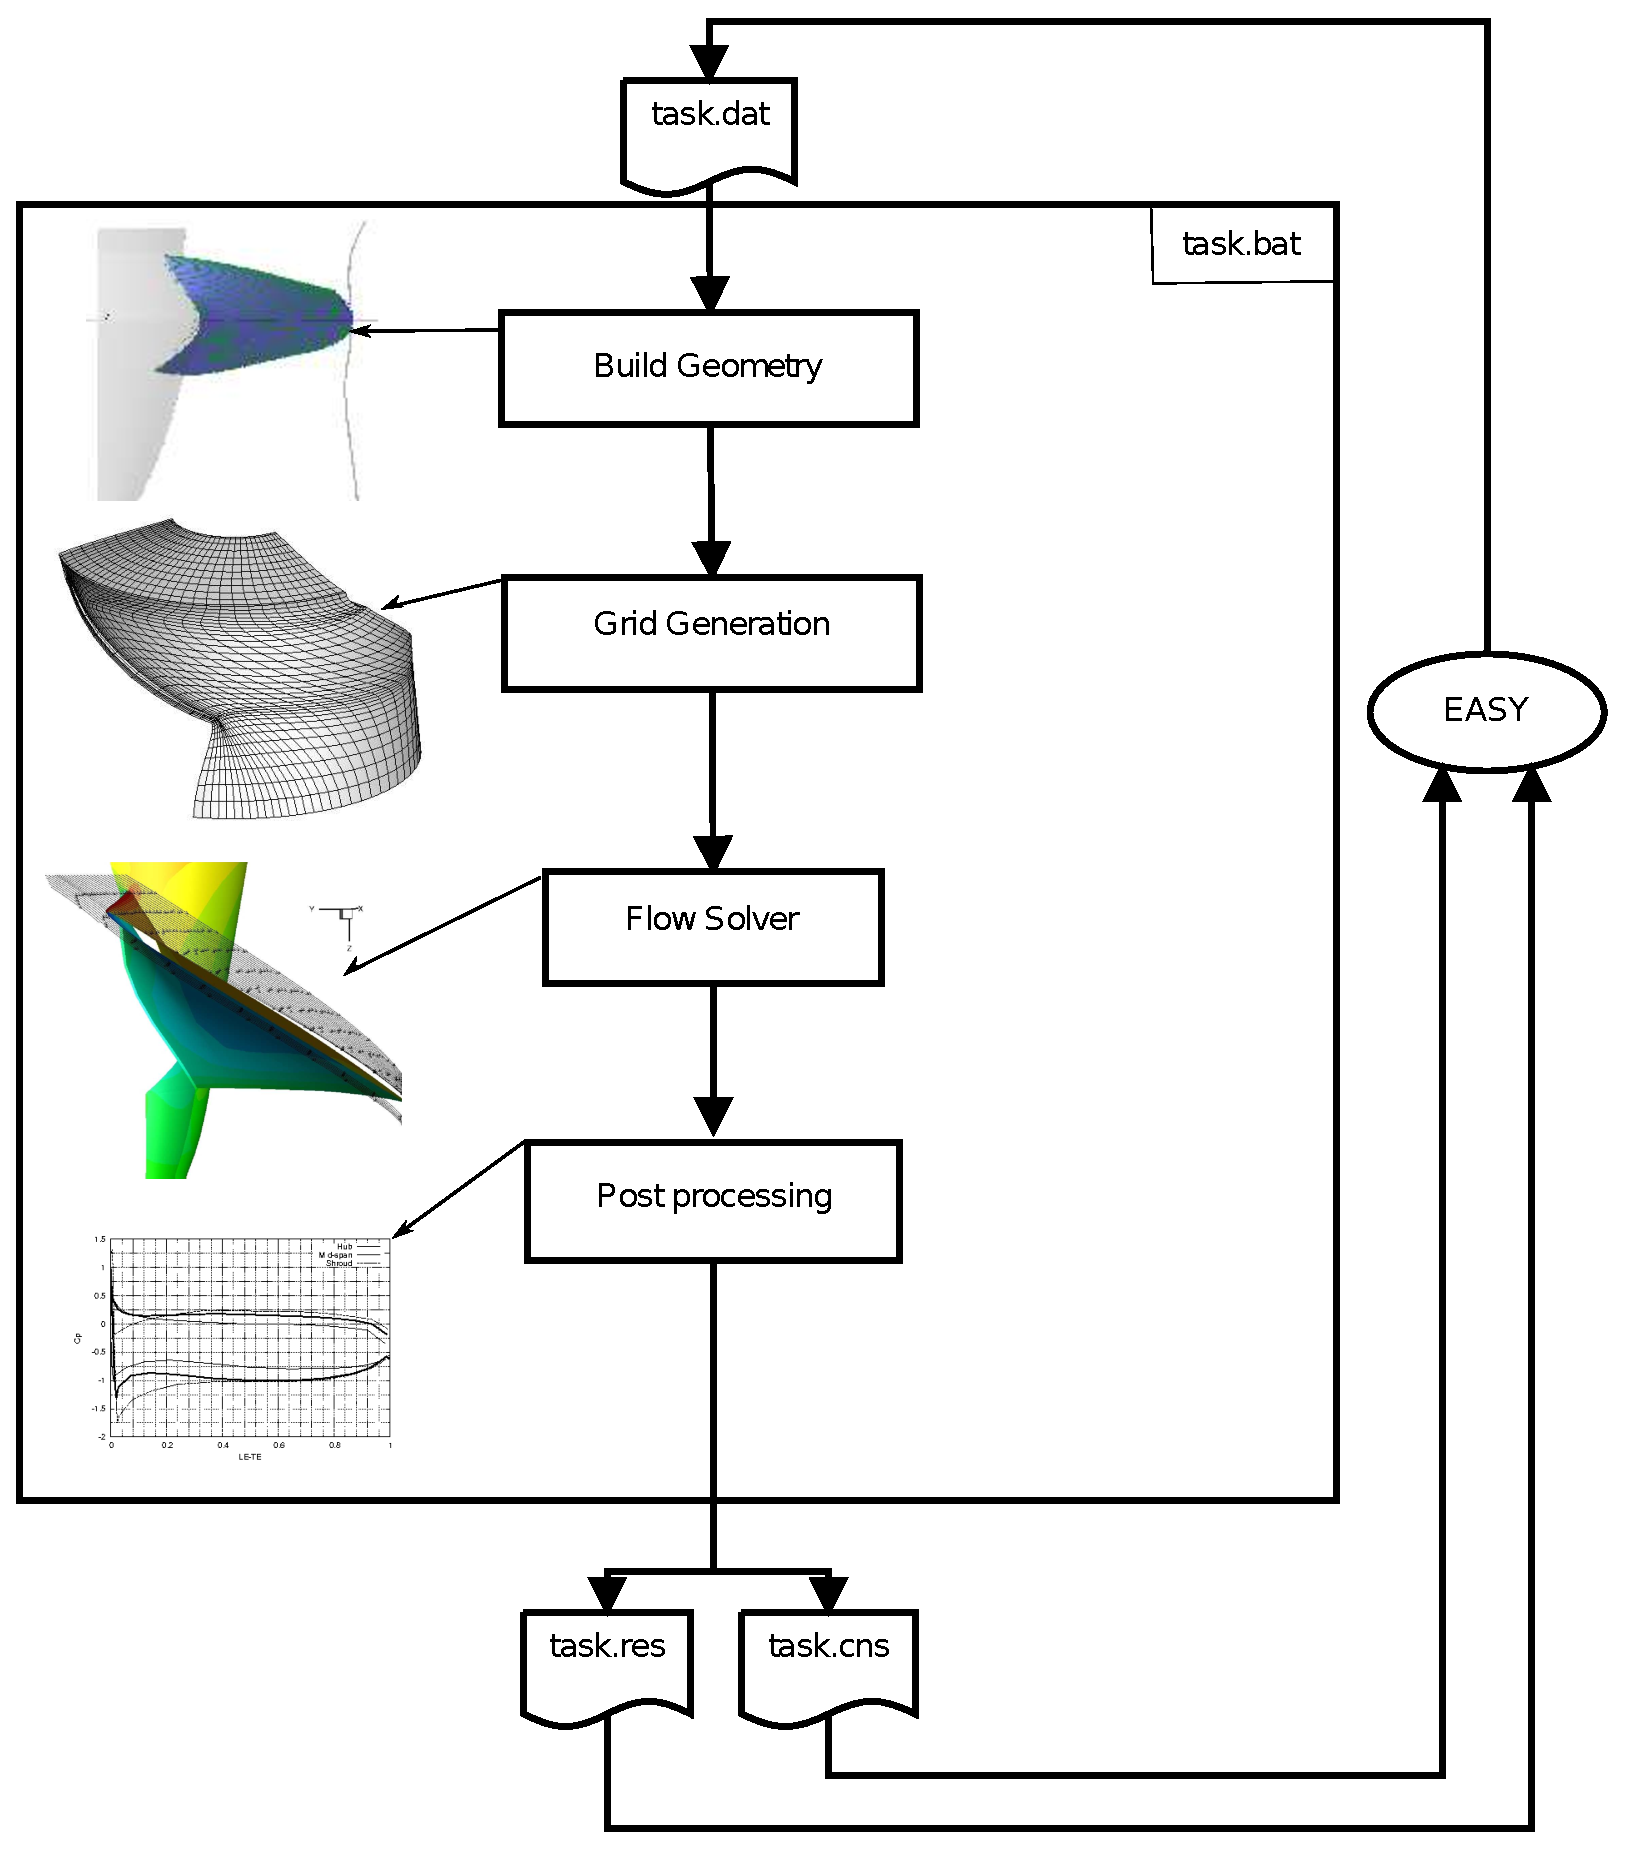
\includegraphics[width=135mm]{Optimizationloop.eps} 
\caption{According to the EASY nomenclature, the evaluation of each new candidate solution provided during the evolution starts by reading the corresponding values of the design variables from the "task.dat" file. A series of codes, being I/O compatible, are sequentially used to finally create the "task.res" and "task.cns" files which indicate the objective and constraint function values respectively. A single evaluation process is considered to be terminated once the "task.res" and "task.cns" files  become available to the search engine of EASY. The executable files required for a single evaluation are listed in the script file "task.bat". }
\label{evaltool}
\end{figure}      
      
\section{Evaluation procedure}
\label{ParamEval}
\subsection{Parameterization for turbine blades}
\label{Paramt}
The  parameterization of a hydraulic turbine blade, either of axial, radial or mixed flow type, consists of two steps. First step is the parameterization of the 3D mean camber surface. The second step is concerned with the thickness of the blade which is defined by the airfoil shape and the thickness distribution across the blade \cite{dipl_livia,dipl_simon}.

Starting point of the parameterization of the mean camber surface is its meridional projection. The meridional projection of the mean camber surface is confined by 4 curves, namely the hub and shroud generatrices and the leading and trailing edge curves (fig.\ref{param1}). All four curves are parameterized by a user defined number of Bezire points.


%\begin{figure}[h!]
%\centering
%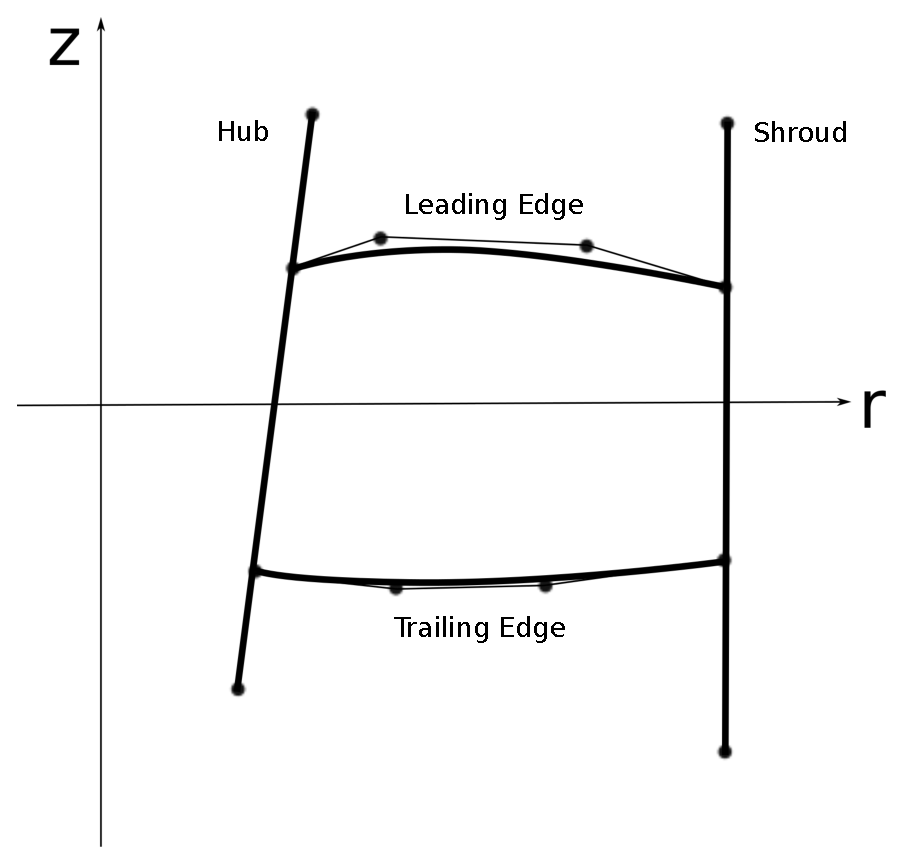
\includegraphics[width=100mm]{param1.eps} 
%\caption{Example of a meridional surface (here a Matrix blade) in cylindrical coordinates (r,z,f=0)}
%\label{param1}
%\end{figure}

Having defined the meridional projection of the mean camber surface, next step is the generation of the 3D shape of the mean camber surface. A set of 2D iso-span lines, distributed between shroud and hub on the meridional surface, are constructed (fig.\ref{param1}). The 3D shape of the aforementioned lines is constructed based on their meridional projection and a number of parameters, namely $\rho,\theta,\beta,\zeta$ and $\mu$ which are all defined below. These 3D lines are then used as the skeleton of the blade mean camber surface (fig.\ref{param3}).

\begin{figure}[h!]
\begin{minipage}[b]{0.5\linewidth}
 \centering
 \resizebox*{6.5cm}{!}{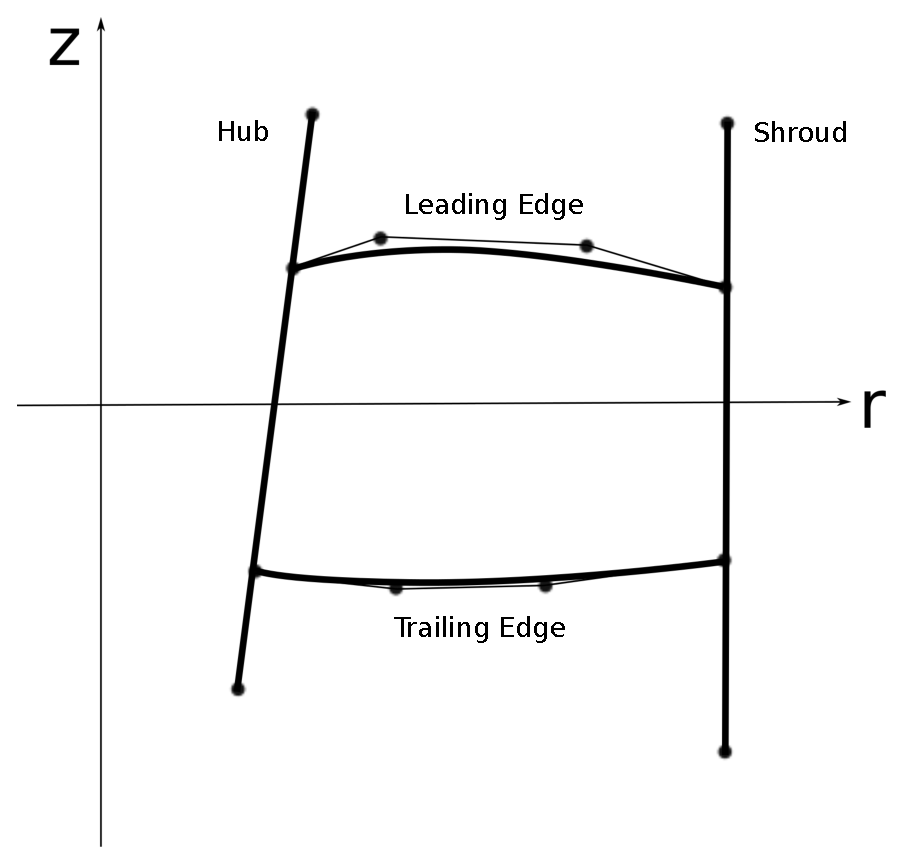
\includegraphics{param1.eps}}
\end{minipage}
\begin{minipage}[b]{0.5\linewidth}
 \centering
 \resizebox*{6.5cm}{!}{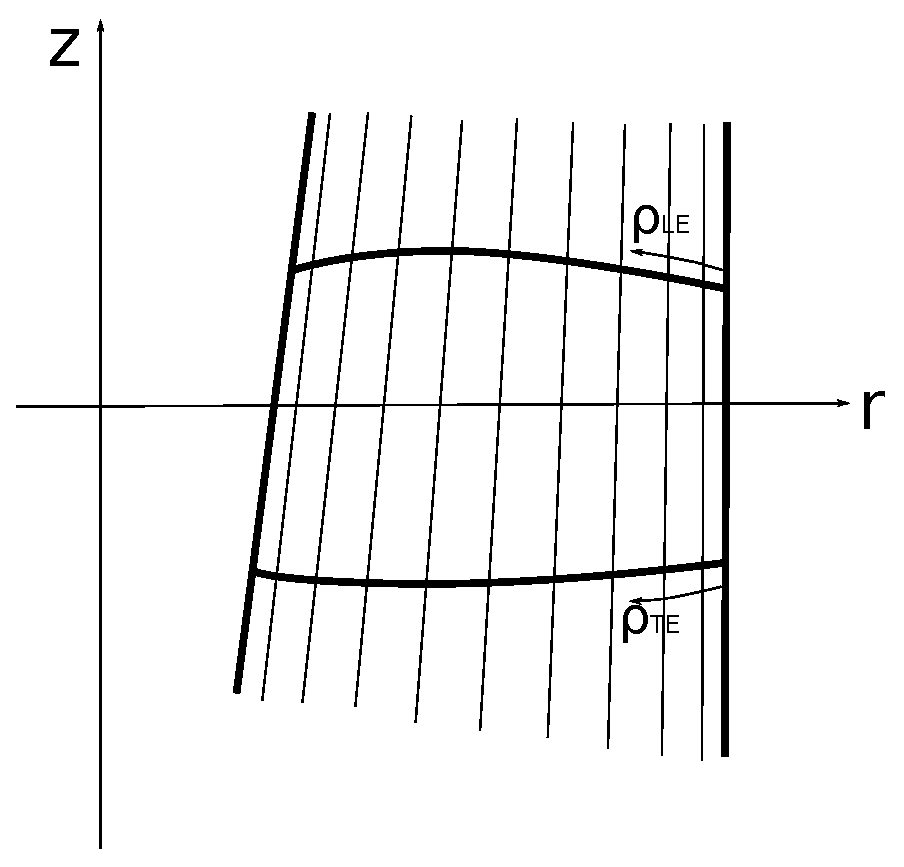
\includegraphics{param2.eps}}
\end{minipage}
\caption{Left; Meridional projection of the mean camber surface of a HYDROMATRIX$\circledR$ blade. Right; The 2D iso-span lines distributed between shroud and hub (here 11 lines). Definition of $\rho$ for the leading and trailing edge.}
\label{param1}
\end{figure}
 

%\begin{figure}[h!]
%\centering
%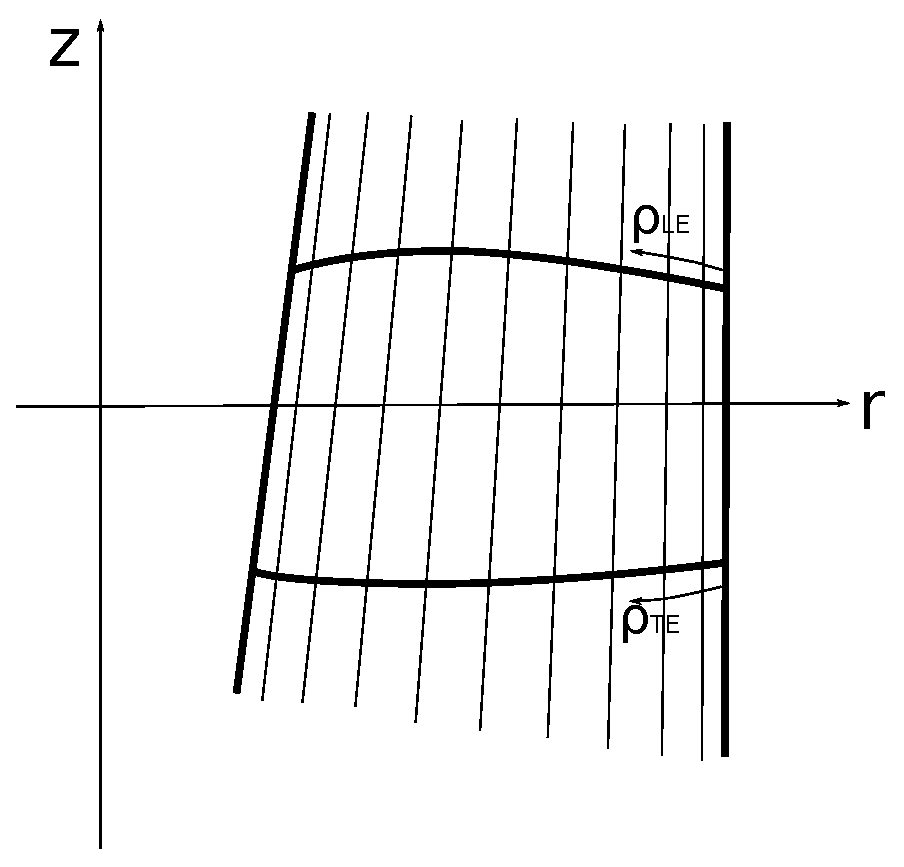
\includegraphics[width=100mm]{param2.eps} 
%\caption{Example of a 2-dimensional streamlines distribution between shroud and hub (here 11 streamlines). %Definition of $\rho$.}
%\label{param2}
%\end{figure}

The $\rho$ value is defined at each point, on both the leading and trailing edge, as the normalized meridional projection arc length of the edge with zero value at the shroud and unity at the hub (fig.\ref{param1}). 

\begin{figure}[h!]
\centering
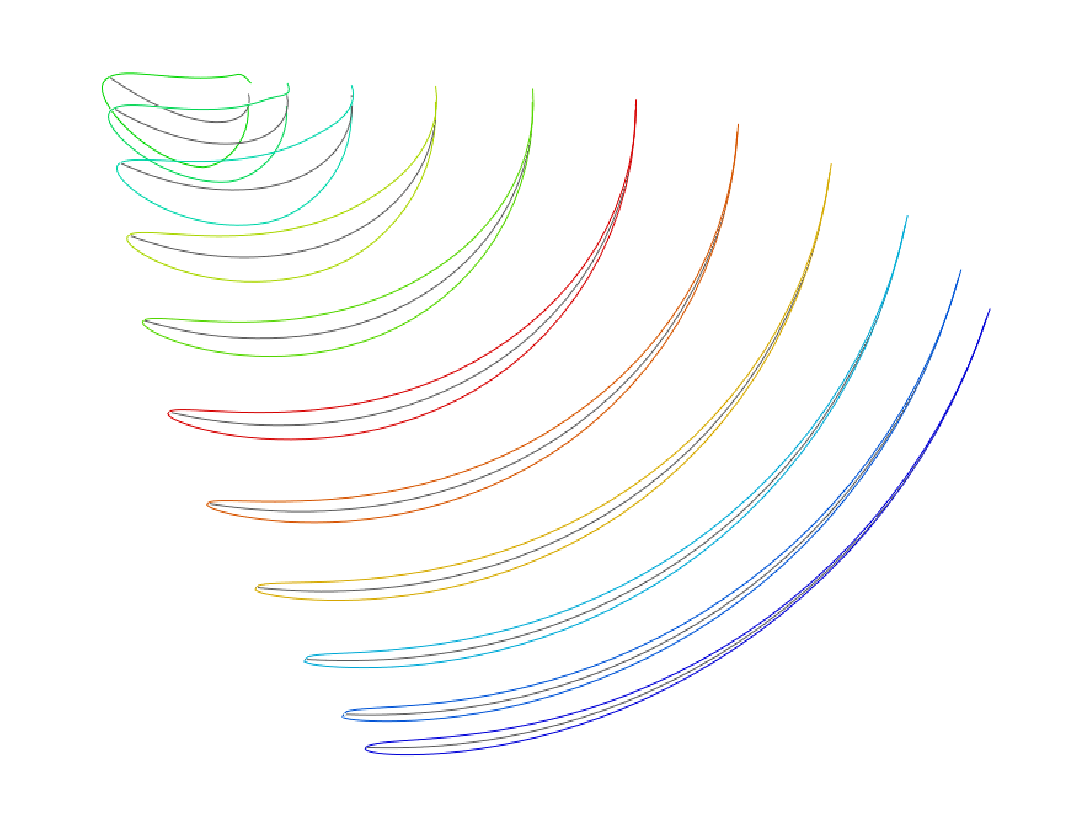
\includegraphics[width=120mm]{param3.eps} 
\caption{The 3D iso-span lines and their superimposed thickness profiles.}
\label{param3}
\end{figure}

The angular position of the leading and trailing edge is controlled by the so-called wrap-around angle ($\theta$). % is defined as the angle between the projected linear connection of a mean-surface-point and the z-axis onto the x-y-plane and the x-axis.
$\theta(\rho)$ distributions for leading and trailing edge together with the r and z values of their meridional projections define the final 3D shape of leading (LE) and trailing (TE) edge. On the other hand $\beta$ is defined as the angle between the local tangent to the mean camber surface and the tangent on the z-centred circle through this point. Therefore $\beta(\rho)$ distributions define the mean camber surface metal angles throughout the previously defined LE and TE. $\beta(\rho)$ and $\theta(\rho)$ distributions are herein parameterized as bezier curves of a user defined degree (fig.\ref{param4}).  


\begin{figure}[h!]
\begin{minipage}[b]{1\linewidth}
 \centering
 \resizebox*{14cm}{!}{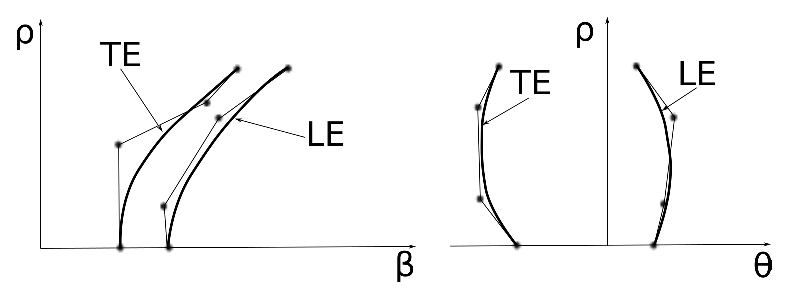
\includegraphics{param4_5.eps}}
\end{minipage}
%\begin{minipage}[b]{0.5\linewidth}
% \centering
% \resizebox*{6.5cm}{!}{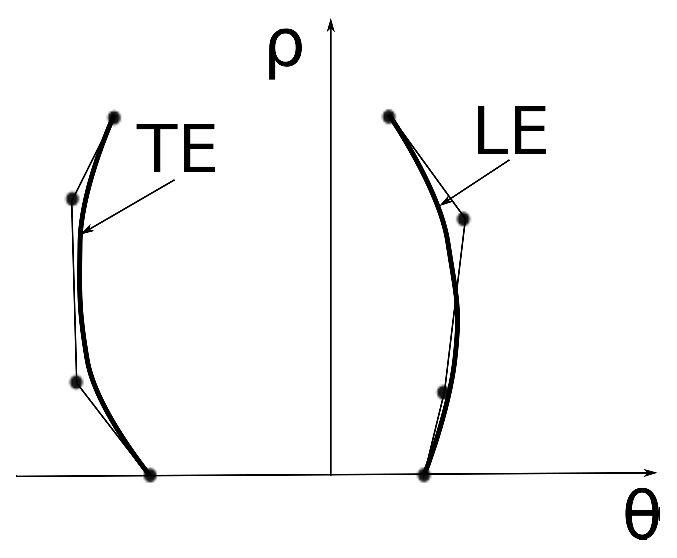
\includegraphics{param5.eps}}
%\end{minipage}
\caption{Left; $\beta(\rho)$ distribution. Right; $\theta(\rho)$ distribution.}
\label{param4}
\end{figure}

The final step in the parameterization of the mean camber surface is to define its shape between leading and trailing edge for all the iso-span lines. This is achieved through the conformal mapping $\Phi$.


\begin{equation} 
   \Phi:(r,z)\rightarrow \mu, ~~~~\mu=\int{\frac{1}{r}dl}
   \label{phi1} 
\end{equation}
where l denotes the arc length of the meridional projection of the iso-span line. This conformal mapping performs the transformation of the iso-span lines from cylindrical coordinates $(r,z,\theta)$ to a $(\mu,\theta)$ coordinate system. Herein the iso-span lines (in the $(\mu,\theta)$ coordinate system) are defined by Bezier curves of third degree. The first and last control points are fixed on the, defined by now, LE and TE points of the iso-span line in hand and the two internal control points depend on $\zeta_{LE}, ~\zeta_{TE}, ~\beta_{LE}$ and $\beta_{TE}$ angles respectively (fig.\ref{param7}).
  
Finally $\zeta(\rho)$ distribution, one for the LE ($\zeta_{LE}$) and one for the TE ($\zeta_{TE}$) define the position of the two internal control points for all the iso-span lines ($0\leq\rho\leq1$). Therefore the $\zeta$ distributions can be seen as the curvature control system of the aforementioned parameterization of the mean camber surface scheme, since it defines how strongly the $\beta$ values at leading and trailing edge will influence the $\beta$ values in the interior of the mean camber surface. Similar to $\theta(\rho)$ and $\beta(\rho)$ also $\zeta(\rho)$ distributions are parameterized as Bezier curves of a user defined degree(fig.\ref{param7}). The inverse conformal mapping $\Phi^{-1}$ is then used to transform the iso-span lines from the $(\mu,\theta)$ coordinate system back to the cylindrical coordinate system. 

\begin{figure}[h!]
\begin{minipage}[b]{1\linewidth}
 \centering
 \resizebox*{14cm}{!}{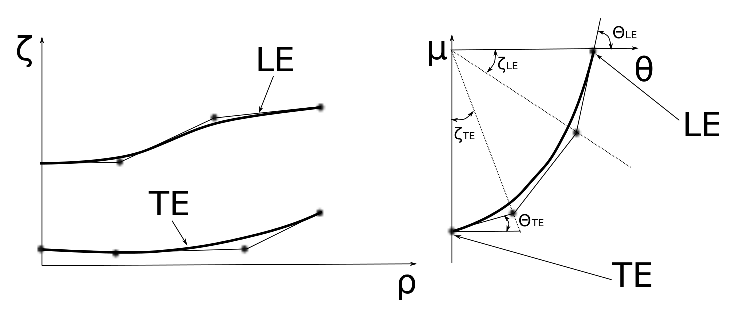
\includegraphics{param6_7.eps}}
\end{minipage}
%\begin{minipage}[b]{0.5\linewidth}
% \centering
% \resizebox*{7.5cm}{!}{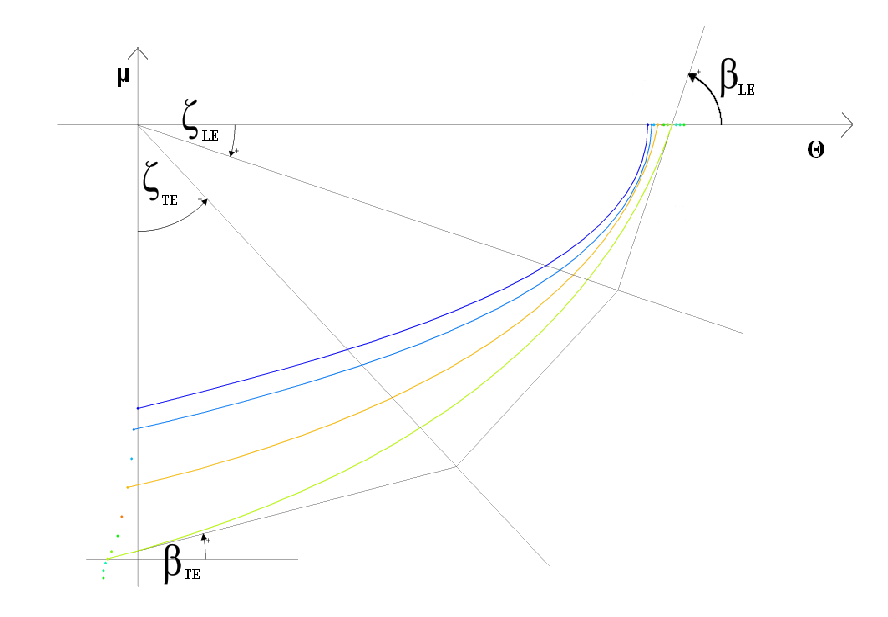
\includegraphics{param7.eps}}
%\end{minipage}
\caption{Left; $\zeta(\rho)$ distributions for $\zeta_{LE}$ and $\zeta_{TE}$. Right; Iso-span line, in $(\mu,\theta)$ coordinate system, and its Bezier control point polygon.}
\label{param7}
\end{figure}

The airfoil profiles are defined by a, user defined, number of Bezier points (fig.\ref{param8}) and the absolute thickness by two thickness (t($\rho$)) distributions (fig.\ref{param10}) (one for the SS and one for the PS). Airfoil profiles are scaled so their maximum thickness is equal to the one specified by the t($\rho$) distribution. The scaled airfoil profiles are then superimposed onto the mean camber surface to create the final 3-dimensional geometry (fig.\ref{param10}).  

\begin{figure}[h!]
\centering
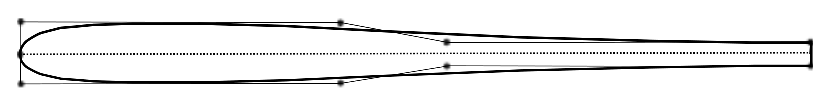
\includegraphics[width=150mm]{param8.eps} 
\caption{Bezier control point polygon regarding the suction side of the airfoil profile. The same paremerization is performed also for the pressure side of each profile. The mean camber surface holds its properties only if the suction and pressure side profiles are symmetrical and the thickness profiles for both SS and PS identical, other wise the mean camber surface transforms into the so-called middle surface.}
\label{param8}
\end{figure}

%\begin{figure}[h!]
%\centering
%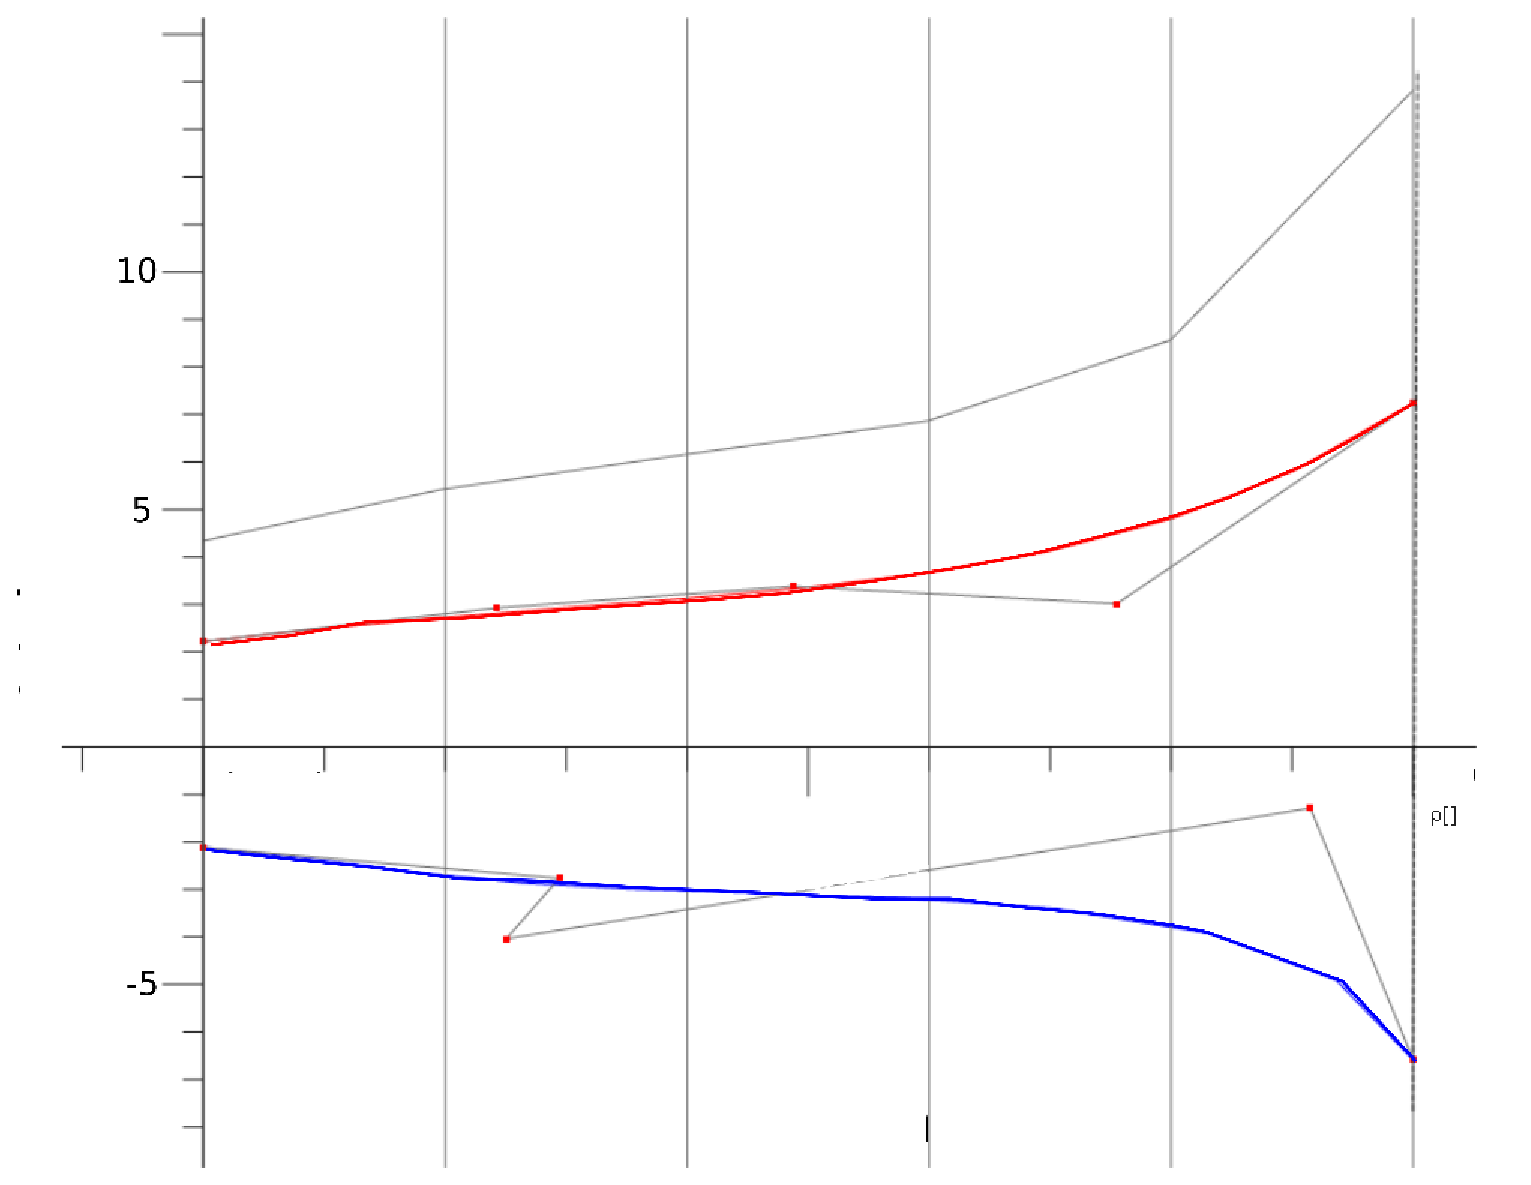
\includegraphics[width=60mm]{figure5.eps} 
%\caption{thickens-$\rho$ distribution.}
%\label{param9}
%\end{figure}


\begin{figure}[h!]
\begin{minipage}[b]{0.5\linewidth}
 \centering
 \resizebox*{6.5cm}{!}{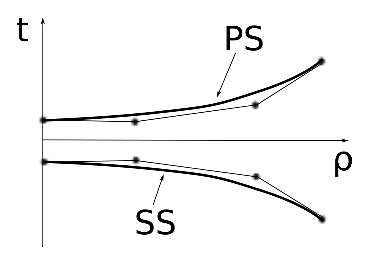
\includegraphics{param9.eps}}
\end{minipage}
\begin{minipage}[b]{0.5\linewidth}
 \centering
 \resizebox*{6.5cm}{!}{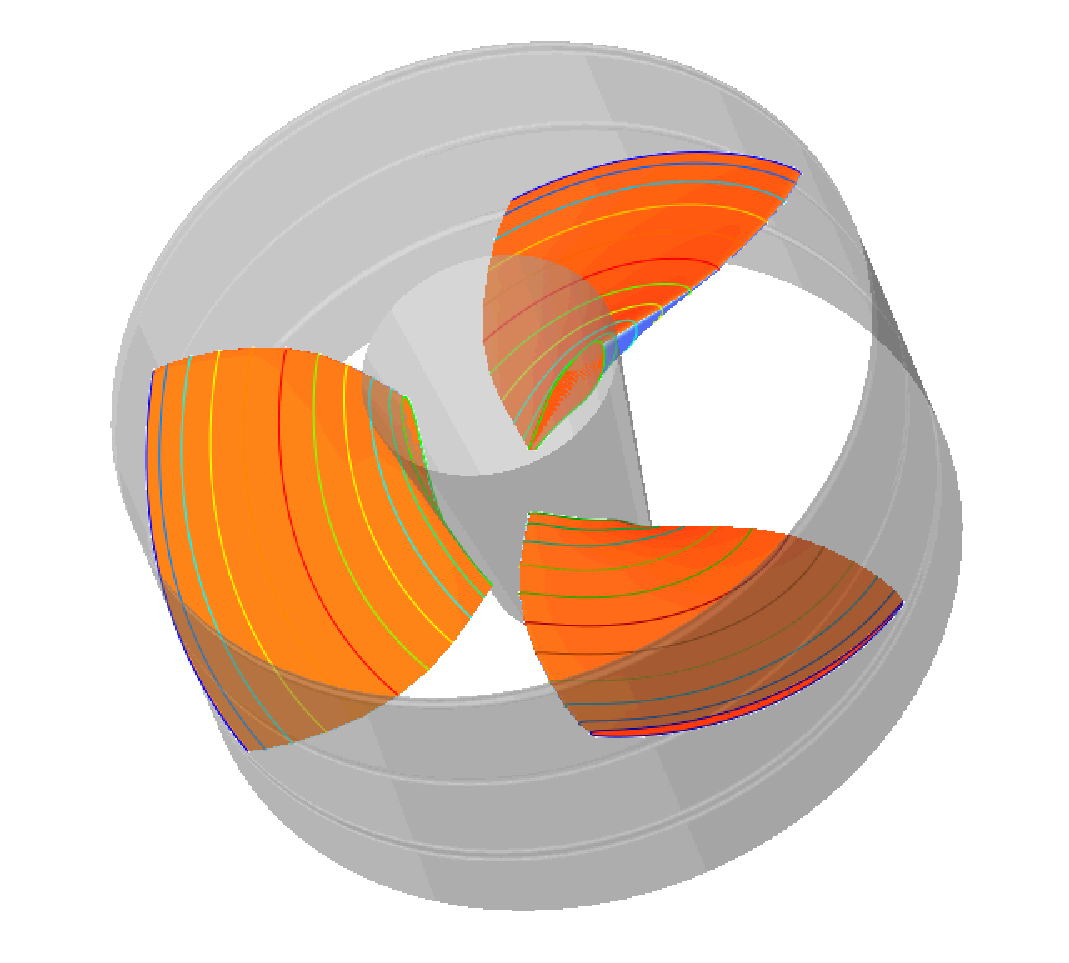
\includegraphics{param10.eps}}
\end{minipage}
\caption{Left; t($\rho$) distribution. Right; 3D geometry of a three bladed HYDROMATRIX$\circledR$ turbine.}
\label{param10}
\end{figure}

\subsection{Space discretization - Grid generation}
\label{SpaceDisct}
A tailor-made for hydraulic turbomachines, able to handle axial, radial and mixed flow machine, multi-bloc structured grid generator is used in this thesis. Structured grids, based on the notion of blocks with fixed topology, can, via stretching and twisting them, create grids that fit a given  body. A multi-block topology (several interconnected structure grid blocks) allows the user greater freedom in constructing grids around complex geometries (fig.\ref{grid1}). 


\begin{figure}[h!]
\centering
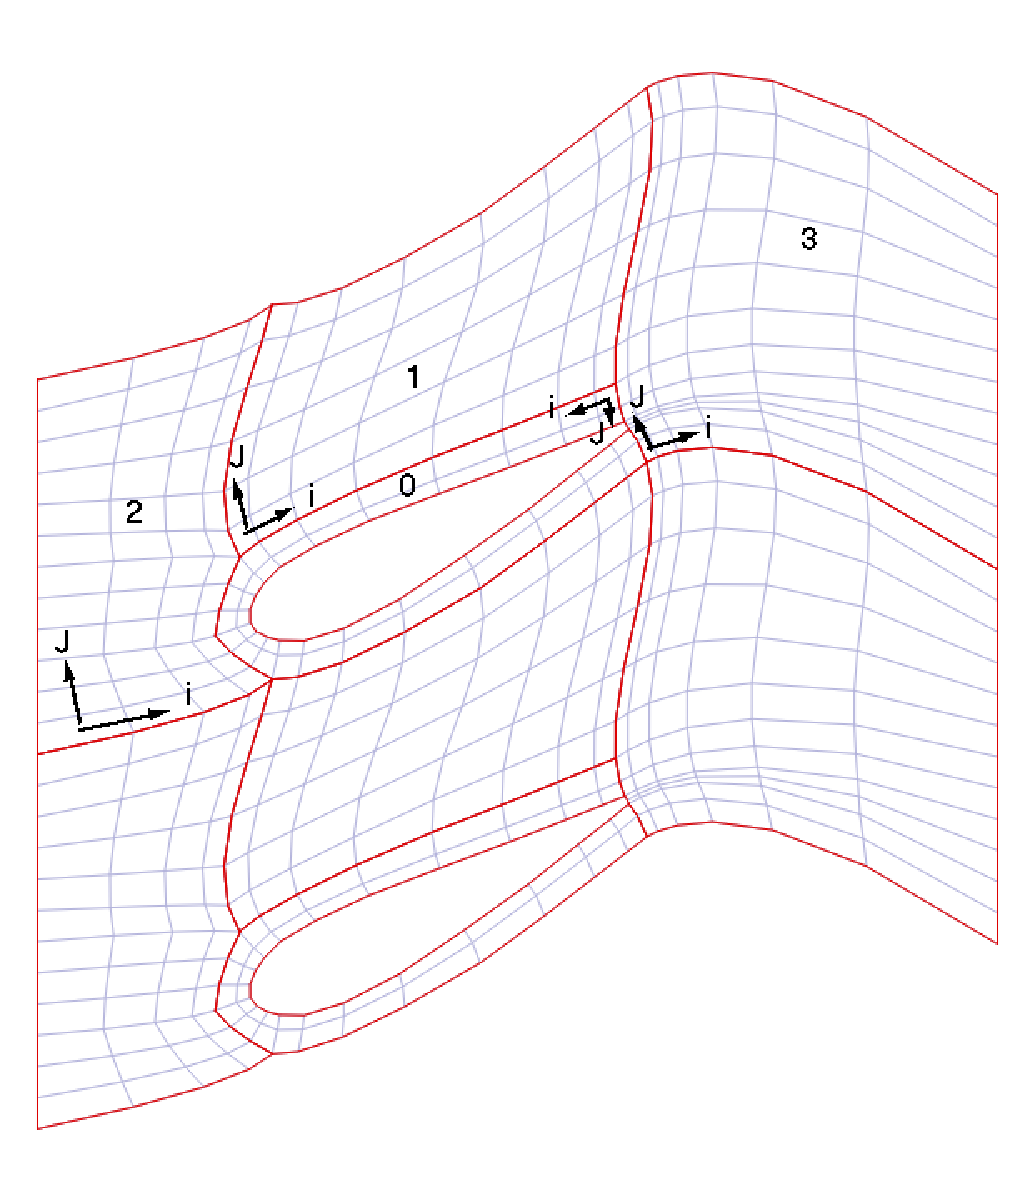
\includegraphics[width=100mm]{cGridSkBlockIndex.eps} 
\caption{The four-block topology of a hydraulic turbine. In the sake of simplicity, this is shown on the blade-to-blade grid at mid-span. Block 0 is of C-type and is used to discretize the area in the vicinity of the blade (herein airfoil). Blocks 1 to 3 are of rectangular type and are used to fill the space from pressure side to suction side, between blade LE and inlet and  blade TE and outlet respectively. }
\label{grid1}
\end{figure}


In this thesis, with respect to the topological characteristics of hydraulic turbo-machines, such as the the TE thickness and the extensions towards the inlet and outlet of the domain, a four block topology is used  fig. \ref{grid1}. Block 0 is used to mesh the area in the vicinity of the blade, capturing the TE thickness, and is of C-type. Block 1 fills the space between two consecutive blades. Block 2 fills the space from the inlet to the blade LE and Block 3 fills the space after blocks 0 and 1 up to the outlet. 

Here the user may control the grid via changing the shape of the block edges, defining number of nodes at each location (fig.\ref{grid2}) and  the distribution of grid-nodes at the domain-borders (fig.\ref{grid3}).                      


\begin{figure}[h!]
\centering
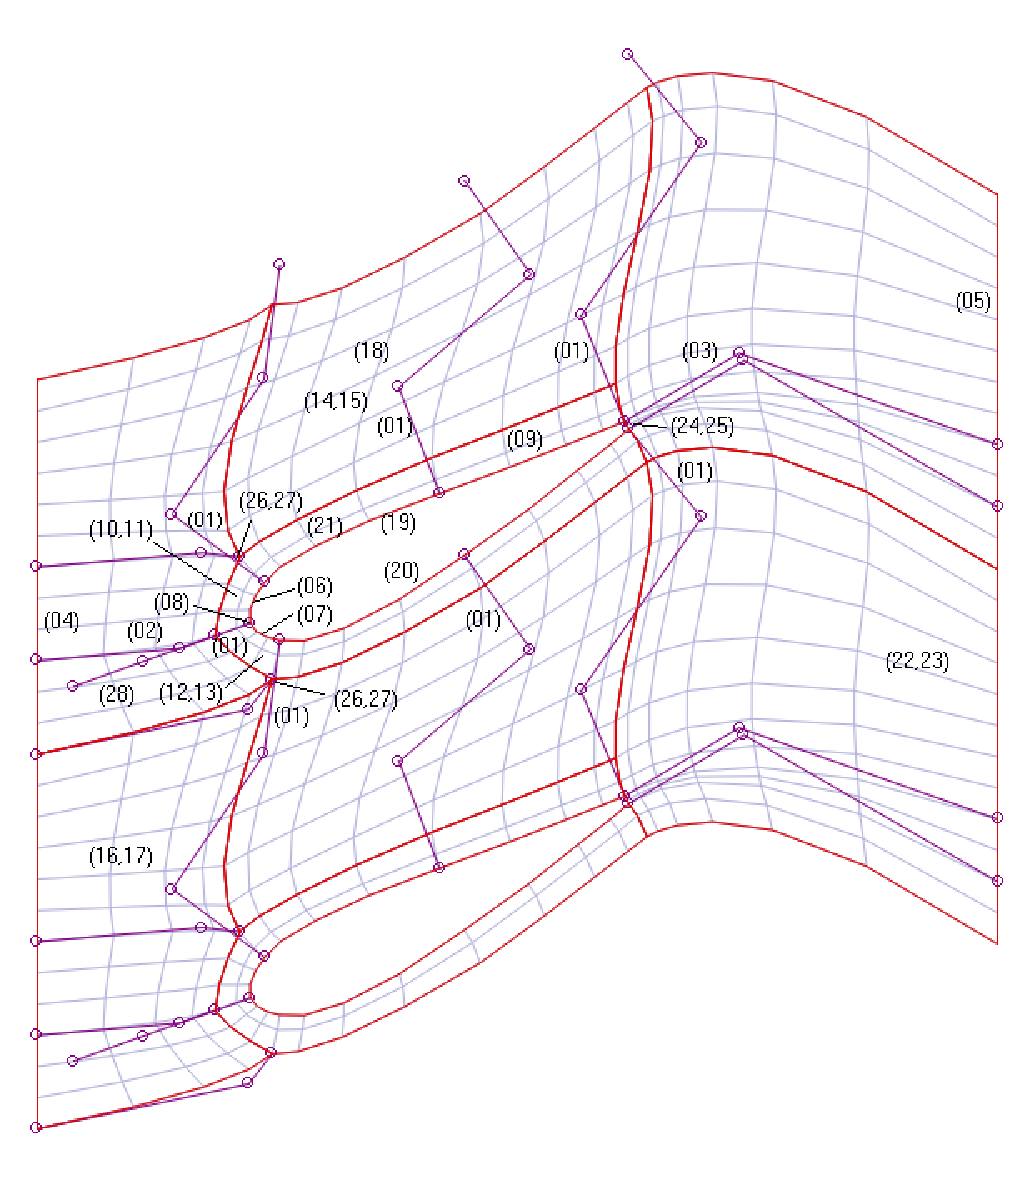
\includegraphics[width=100mm]{cGridSkParam.eps} 
\caption{User-defined parameters controlling the shape of the block edges. These are a set of values constructed from a number of angles and distances that defined the control points of the figure. Numbers on these figure correspond to the number of the parameters and are depicted in the domains that they influence.}
\label{grid2}
\end{figure}

\begin{figure}[h!]
\centering
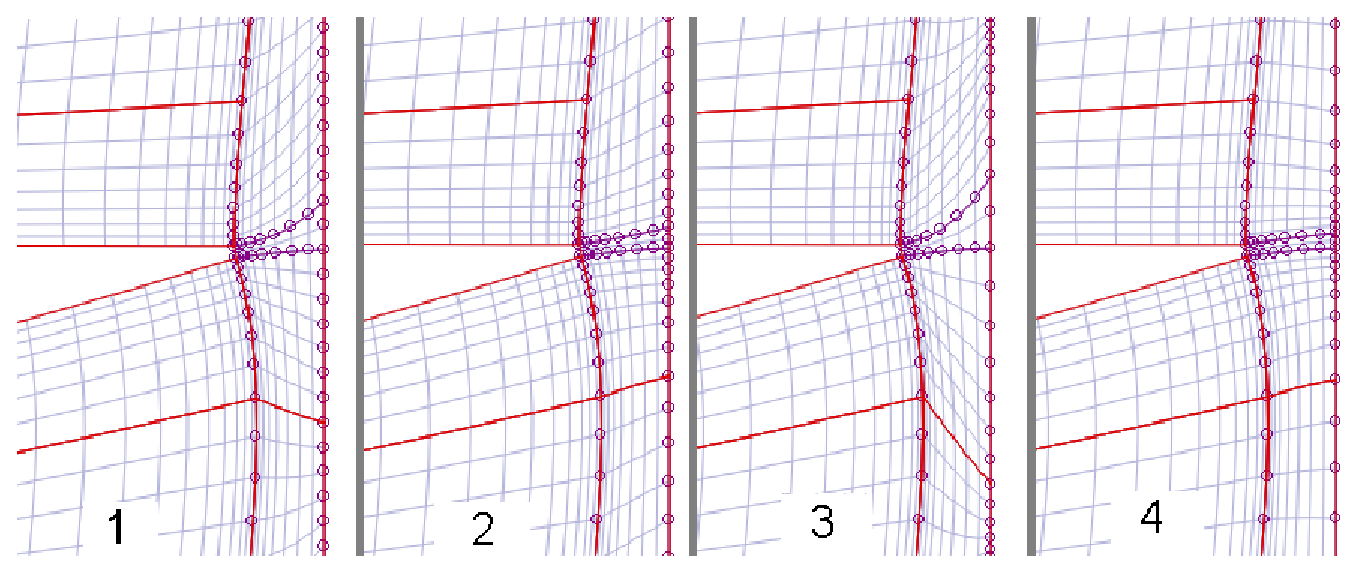
\includegraphics[width=120mm]{sketchDistrEast.eps} 
\caption{Parameters controlling the distribution of grid-nodes along the domain-boundaries allow the user to place a greater number of points in regions of high gradients while reducing the number of grid nodes in regions with small gradients.}
\label{grid3}
\end{figure}

To construct the three-dimensional grid a user-defined number of pseudo two-dimensional (laying on iso-span surfaces fig \ref{grid4}) grids are computed using the grid parameterization as described above and are then combined to create the final 3D grid.

\begin{figure}[h!]
\centering
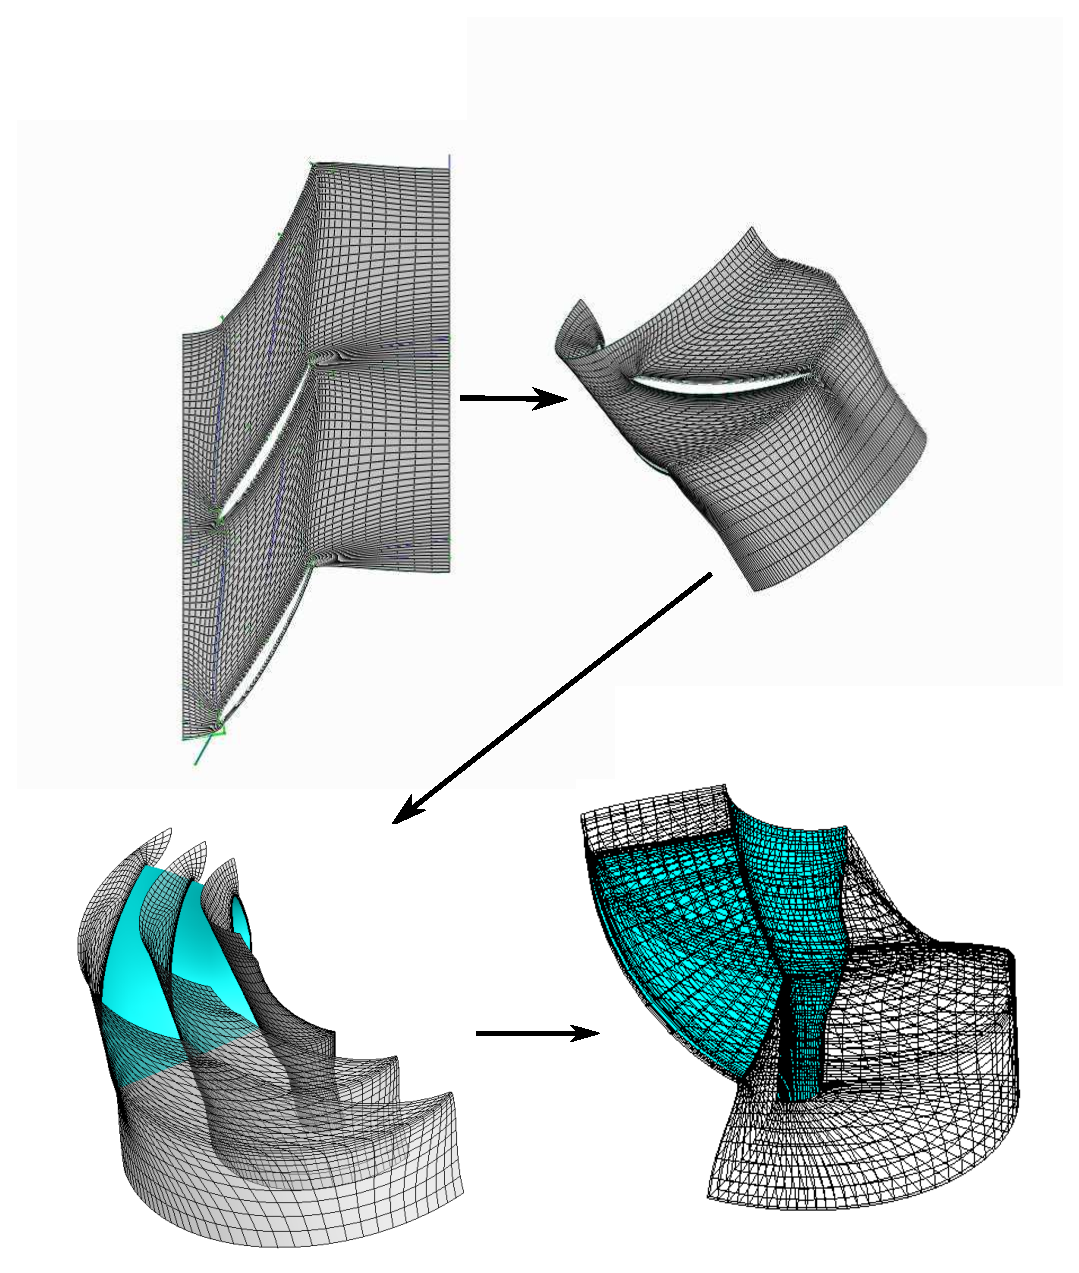
\includegraphics[width=140mm]{merid.eps} 
\caption{Iso-span surface grid as pseudo-2D grid. A user-defined number of the iso-span surface grids (from hub to shroud) is combined in order to generate the three-dimensional grid. Top Left: the pseudo-2D grid at the mid-span position. Top Right: the same grid transformed buck to the 3D space. Bottom Left: The hub: mid-span and shroud grids. Bottom Right: Final grid.}
\label{grid4}
\end{figure}

It is important to mention that the described grid generation technique can accommodate a great variation of geometries without failing. This is with great importance for a grid technique to be used in an optimization framework. Good geometries should under no circumstances be classified as "failed" due to the failure of the grid generation process. 

In this thesis both, guide vane and runner blade channels are meshed using a grid generation tool, with the previous features, developed by Andritz-ASROE. 
%Typically, for speed sake, only one circumferential channel is computed (one guide vane and one runner channel with mixing plane interface).  


\subsection{Flow Solver}
\label{FlowSolvert}
Water flow through the hydraulic turbine blades is simulated by a CFD code developed by Andritz-ASROE (cite Arno G1+ literature). The aforementioned code is a multiblock solver for incompressible 3D euler flow. The Euler (eq. \ref{Euler1}) equations are expanded by an artificial compressibility, the solution is achieved, using the 1D Roe approximate Riemann solver \cite{Roe81}, iteratively by ADI (alternating direction implicit) method on structured grids. Convergence is accelerated by a V-cycle multigrid schema. The solver is developed for hydraulic turbomachines, rotational axis is z-axis.

%using the 1D Roe approximate Riemann solver \cite{Roe81}
%is solving the Euler equations (eq. \ref{Euler1}) based on the artificial compressibility approach using the 1D Roe approximate Riemann solver \cite{Roe81}. For sake of wall time reduction this code employs a multi-grid solver. 

In differential form the Euler equations (artificial compressibility approach) are;
\begin{equation} 
    \frac{\partial Q}{\partial t}=\nabla \cdot F
	\label{Euler1}
\end{equation}

where,
\begin{eqnarray}
		Q= \left( {\begin{array}{c}
 		p    \\
 		u_1  \\
 		u_2  \\
 		u_3  \\
 		\end{array} } \right)
 		F_i= \left( {\begin{array}{c}
 		\beta ^2 u_i    \\
 		\beta ^2 u_1u_i + p\delta _1^i  \\
		\beta ^2 u_2u_i + p\delta _2^i  \\
 		\beta ^2 u_3u_i + p\delta _3^i  \\
 		\end{array} } \right)
\label{Euler3}
\end{eqnarray} 
 
where $\beta$ the artificial compressibility \cite{Chorin,Turkel87} and $\delta^i_j$ the Kronecker symbol.

%Using the above formulation each CFD calculation inside one runner channel takes only a few minutes. This fact and the observation that the influence of turbulence and viscosity are small enough allows, in combination with the proposed in this thesis techniques, the use of EAs as design tools in an industrial level i.e. with short (acceptable in a industrial environment) wall time. 

%Of coarse for the above statement to be true the appropriate objective functions, derived out of quality metrics that reflect the real quality of a runner and are not significantly influenced by turbulence and viscosity, have to be chosen. This type of metrics are presented, in detail, in section \ref{metrics} and will be used throughout this chapter. 
 
%In order to eliminate the obvious problem for incompressible flow (reduced state equation) an %artificial compressibility is introduced (cite R2 S5 ,maybe more). 

%The term $\frac{\partial \rho}{\partial t}$ is expanded by $\frac{\partial p}{\partial p}$, which results in 


%\begin{eqnarray}
%	\frac{\partial \rho}{\partial t} = \frac{\partial \rho}{\partial t}\frac{\partial p}{\partial p}
% = \frac{\partial p}{\partial t}\frac{1}{(\frac{\partial p}{\partial \rho})} 
% = \frac{\partial p}{\partial t}\frac{1}{\beta ^2}    
%\end{eqnarray}

%Thus the artificial compressibility $\beta$ is defined as;

%\begin{eqnarray}
%	\beta=\sqrt{\frac{\partial p}{\partial \rho}}
%\end{eqnarray}



\section{Hydraulic turbine-runner quality metrics}
\label{metrics}
Metrics are used in order to quantify the quality of candidate solutions. A metric may coincide with a objective function or part of an objective function or a constraint used in the optimization problem.

In this thesis metrics are associated with:
\begin{itemize}
\item{\textbf{$\sigma$:}} The cavitation behaviour of the blade in hand; cavitation is a common problem of all hydraulic machine subject to low pressure liquids, causing performance degradation and structural damages.
\item{\textbf{M1}} The Circumferential and meridional velocity profiles at the exit position of the runner; the exit of the runner coincides with the inlet to the draft-tube and these profiles significantly affect the matching of the two components.
\item{\textbf{M2}} The blade loading quality, since equidistributed loading is desired along the chordwise direction of the blade at any span-wise location.
\item{\textbf{M3}} The pumping surface of the blade; in case of non-regulated turbines neither the stator nor the rotor blade can be rotated/adjusted to operate optimally at every operating point. In such a case, during  part load operation, a small part of the blades surface is operating as a pump, i.e. pressure side has lower pressure than suction side, this surface is desired to be minimized.
\end{itemize}


\subsection{Cavitation metric}
Cavitation in hydraulic turbines, is the phenomenon of water vaporization (formation of cavities/bubbles) as the pressure tends to become lower than the vapour pressure. When the cavitation bubbles collapse in the vicinity of a solid surface, they can cause erosion, compromising thus both the structural integrity (removed material) and the hydraulic performance (altered shape) of the machine \cite{thiruvengadam1974handbook,knapp1970cavitation,brennen1995cavitation}.  In addition, the collapse of cavitation bubbles generates noise, via the large, momentary, pressures that are generated when the internal of the bubble is highly compressed.

The conventional way to characterize how close the minimum liquid pressure is to the vapour pressure and, therefore, quantify the danger of cavitation to occur, is by means of the so-called cavitation number $\sigma$, defined as,

\begin{eqnarray}
		\sigma=\frac{p_{\infty}-p_{v,T_{\infty}}}{0.5\rho_{L}U^2_{\infty}}
\label{Cavi}
\end{eqnarray}
where, $U_{\infty}$,$p_{\infty}$ and $T_{\infty}$ are a reference velocity, pressure and temperature respectively. $\rho_{L}$ is the liquid density and $p_{v,T_{\infty}}$  is the saturated vapour pressure. 

Clearly if $\sigma$ is sufficiently large, $p_{\infty}$ is large compared with $p_{v,T_{\infty}}$ or $U_{\infty}$, single-phase liquid flow will occur. However, if $\sigma$ drops below the $\sigma$ incipient ($\sigma_i$) value cavitation will occur. In the simplified case of a liquid that cannot withstand any tension and in which vapour bubbles appear instantaneously when minimum pressure ($p_{min}$) reaches $p_{v}$,

\begin{eqnarray}
		\sigma_i=\frac{p_{\infty}-p_{min}}{0.5\rho_{L}U^2_{\infty}}
\label{Cavi2}
\end{eqnarray}
Hence, the incipient cavitation number could be ascertained from observations, measurements or simulations of the single-phase flow i.e. for $\sigma > \sigma_i$ the pressure along the entire flow filed is greater than $p_v$ thus no cavitation occurs. On the other hand, if $\sigma \leq \sigma_i$, it exists at least one point in the flow filed with pressure lower than $p_v$ thus cavitation does occur. 


In the case of hydraulic turbines the tendency of the flow to cavitate is characterized by the so called Thoma cavitation coefficient $\sigma$, 
\begin{eqnarray}
		\sigma=\frac{p_{tot,exit}-p_{v}}{\rho_{L}gH}
\label{Cavi3}
\end{eqnarray}
where $p_{tot,exit}$ is the total pressure at the exit of the turbine, $p_v$ the vapour pressure for the liquid and $H$ the hydraulic turbine head. The denominator is the total pressure difference between the turbines inlet and outlet.   

Making the same assumptions as for eq.\ref{Cavi2} the $\sigma_i$ for the Thomas cavitation coefficient  is, 

\begin{eqnarray}
		\sigma_i=\frac{p_{tot,exit}-p_{min}}{\rho_{L}gH}
\label{Cavi4}
\end{eqnarray}

Let $C_p$ the pressure coefficient for hydraulic turbines be 
\begin{eqnarray}
		C_p=\frac{p-p_{tot,exit}}{\rho_{L}gH}
\label{Cpdef}
\end{eqnarray}

The $\sigma_i$ for the Thomas cavitation coefficient can be described as 
\begin{eqnarray}
		\sigma_i=-C_{pmin}
\label{Cavi6}
\end{eqnarray}
where $C_{pmin}$ is the $C_p$ value at the location with minimum pressure ($p_{min}$).

The cavitation behaviour of a hydraulic turbine can be observed through the $C_p$ distribution as they are plotted over the hydraulic turbine surfaces.  In fig. \ref{design-cav-cp} the $C_p$ distribution regarding the turbine runner blade at mid-span position is depicted. The three indicative scenarios for this case is; a) $\sigma>-C_{pmin}$ thus $p_v<p_{min}$ and therefore cavitation dose not occur; b)  $\sigma=-C_{pmin}$, in which case if the assumptions of eq.\ref{Cavi2} and \ref{Cavi4} are true, the liquid cannot withstand any tension and vapour bubbles appear instantaneously when minimum pressure ($p_{min}$) reaches $p_{v}$, cavitation will occur at the point of minimum pressure; and c) $\sigma<-C_{pmin}$ in which case $p<p_v$ over a portion of the chord, in the case of the chord-wise distribution depicted in fig. \ref{design-cav-cp}, or area, in the case of the complete blade. This region is, therefore, considered cavitated.     

\begin{figure}[h!]
\begin{minipage}[b]{1\linewidth}
 \centering
 \resizebox*{14cm}{!}{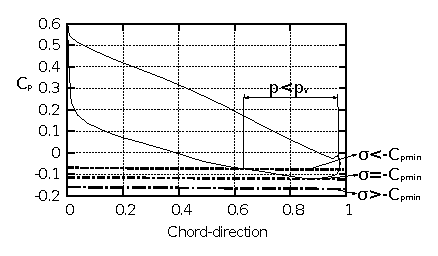
\includegraphics{CP2.eps}}
\end{minipage}
\caption{Pressure coefficient distribution for the mid-span position.}
\label{design-cav-cp}
\end{figure}

In this thesis, in order to reduce the effects of the assumptions of eq.\ref{Cavi2} and eq.\ref{Cavi4}, the $\sigma$-Histogram method \cite{Schmidl} is used. In $\sigma$-Histogram method, during the calculation of $\sigma_i$ the minimum pressure $p_{min}$ is replaced with so called histogram pressure ($p_{Hist}$) (eq. \ref{Cavi7}). $p_{Hist}$ is extracted from the blade pressure distribution where a user-defined surface percentage (A) is required to have pressure values below $p_{Hist}$ fig.\ref{design-cav-histo}.  

\begin{eqnarray}
		\sigma_i^{Hist}=\frac{p_{tot,exit}-p_{Hist}}{\rho_{L}gH}
\label{Cavi7}
\end{eqnarray}
%where

%\begin{eqnarray}
%		A(p<p_{Hist})=A\%A_{Blade}
%\label{Cavi7}
%\end{eqnarray}

\begin{figure}[h!]
\begin{minipage}[b]{1\linewidth}
 \centering
 \resizebox*{14cm}{!}{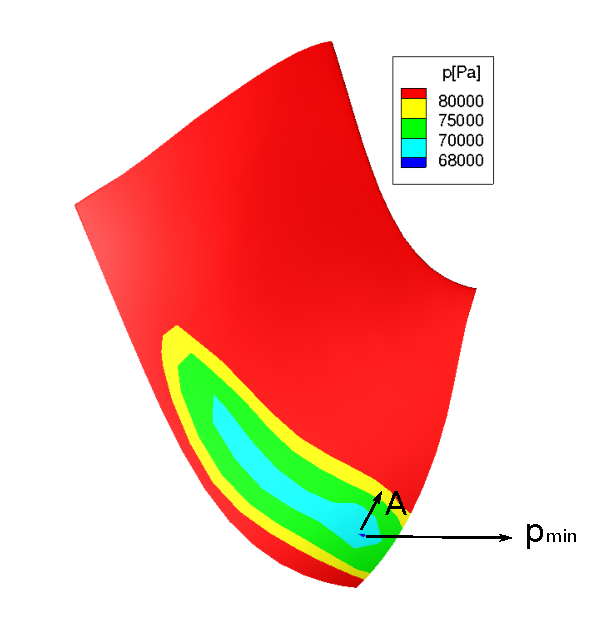
\includegraphics{histo.eps}}
\end{minipage}
\caption{$p_{Hist}$ computed with three different A values is depicted here along side with $p_{min}$ on the suction side of a Francis hydraulic turbine. Increasing A results in increased $p_{Hist}$ and therefore reduced $\sigma_i^{Hist}$. A values in this figure are exaggerated for sake of presentation.}
\label{design-cav-histo}
\end{figure}

%\begin{figure}[h!]
%\begin{minipage}[b]{0.5\linewidth}
% \centering
% \resizebox*{7.5cm}{!}{\includegraphics{sigma.eps}}
%\end{minipage}
%\begin{minipage}[b]{0.5\linewidth}
% \centering
% \resizebox*{6.0cm}{!}{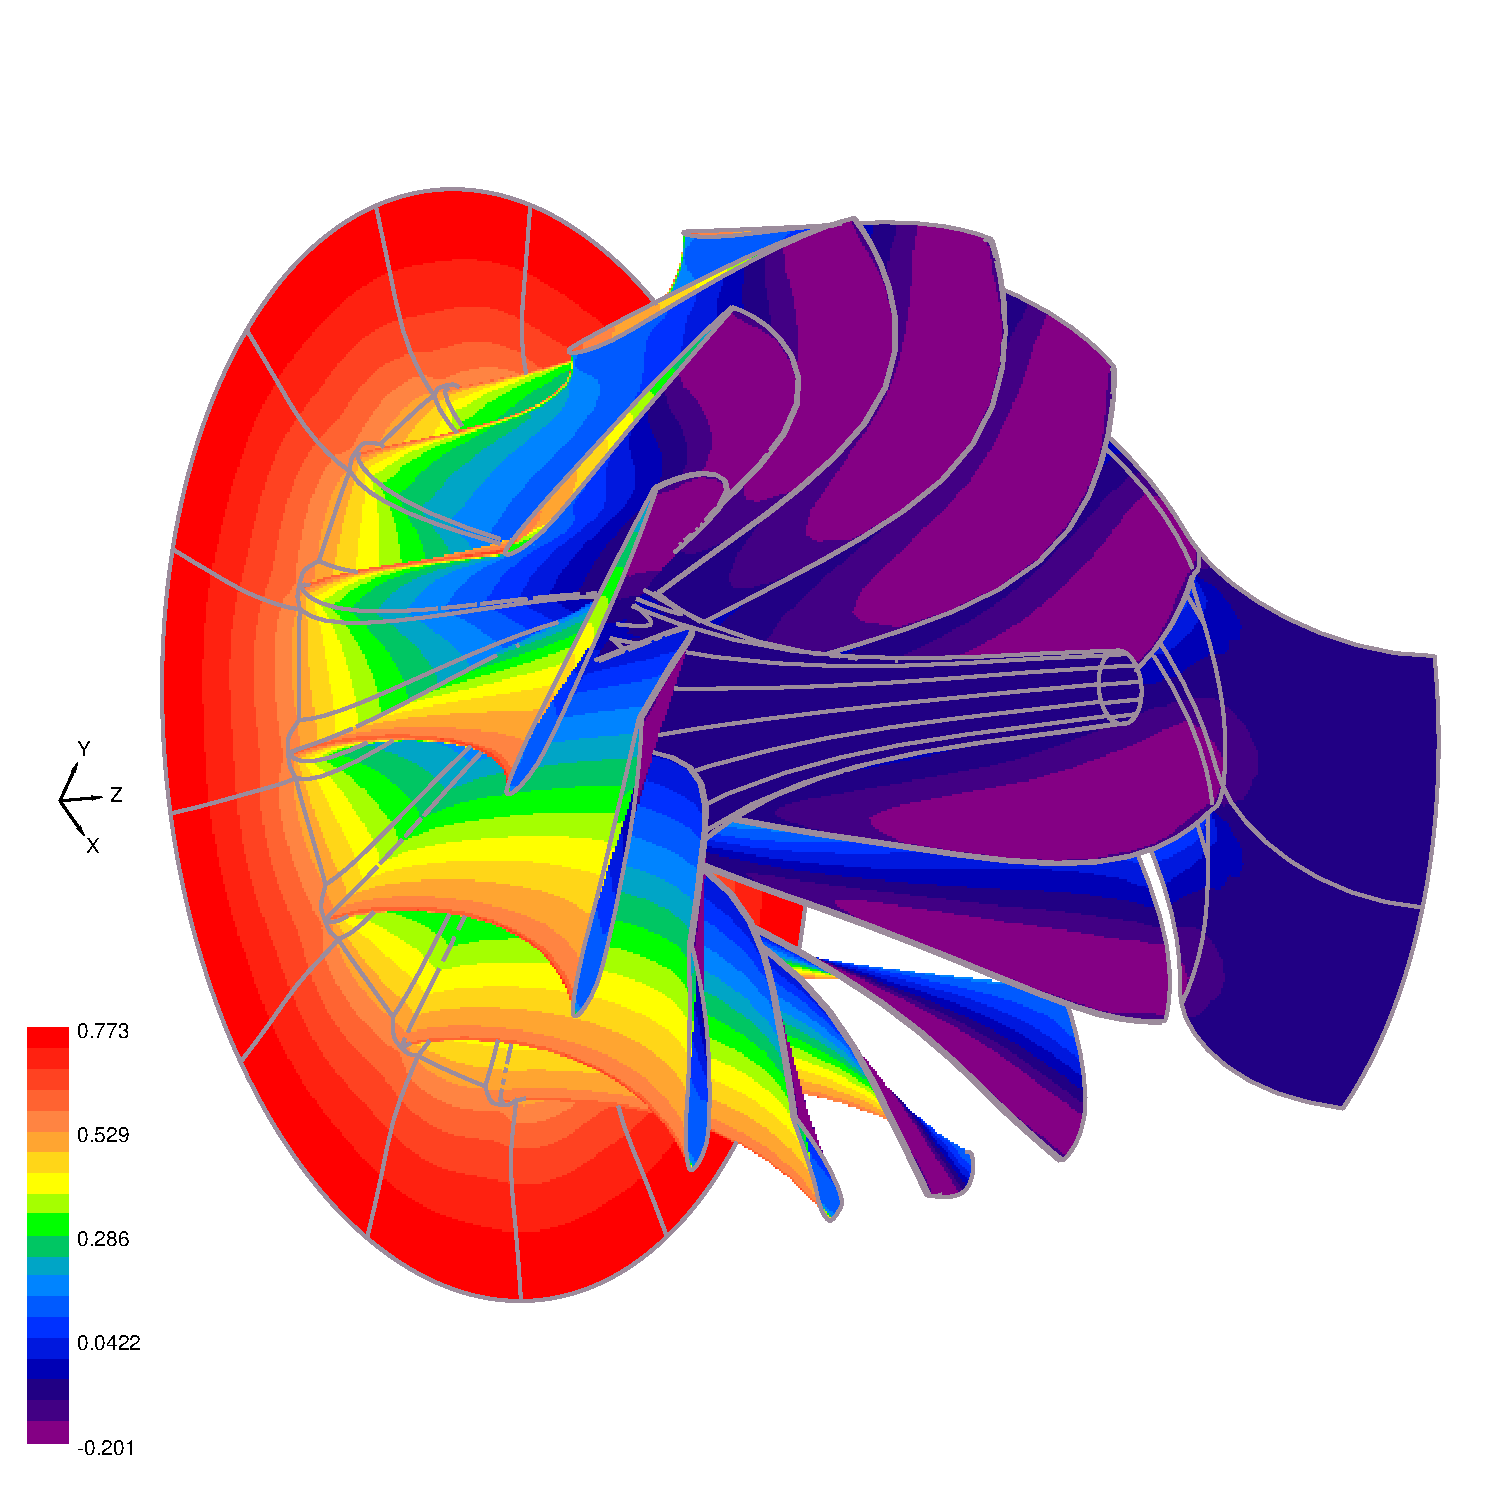
\includegraphics{Cavitation.eps}}
%\end{minipage}
%\caption{Left; $\sigma_{histogram}$ is equal to the $\sigma$ value for which a specific percentage of the blades surface "A" has lower pressure values than $p_{Hist}$, here A is set equal to $0.2\%$ of the blades surface, A is the blade surface that corresponds to the gray area here; Francis runner $\sigma$ contour plot. }
%\label{design-cav}
%\end{figure}


\subsection{Outlet velocity profiles}
Coupling the turbine runner with a pre-existing draft-tube is controlled via the outlet velocity profile metrics. This requires the definition of a target distribution and, thus, the corresponding metric stands for the deviation of the acquired distribution from the target one (fig.\ref{design-obj2}). To perform optimally, a given draft-tube must have, at its inlet, a specific mass-flow ($C_m=\frac{c_m}{\sqrt{2gH}}$) and  specific swirl ($C_u=\frac{c_u}{\sqrt{2gH}}$) span-wise distribution where, $c_m$ and $c_u$ are the meridional and circumferential components of the flow velocity respectively.

%\begin{eqnarray}
%		C_m=\frac{c_m}{\sqrt{2gH}}
%\label{Cavi4}
%\end{eqnarray}
%and 
%\begin{eqnarray}
%		C_u=\frac{c_u}{\sqrt{2gH}}
%\label{Cavi4}
%\end{eqnarray}
%where $c_m$ and $c_u$ are the meridional and circumferential components of the flow velocity respectively.

Therefore the  "outlet quality" optimization objective is defined as minimization of the deviation between the acquired distributions and the corresponding target. 

\begin{figure}[h!]
\begin{minipage}[b]{1\linewidth}
 \centering
 \resizebox*{10.0cm}{!}{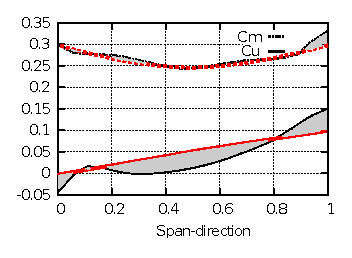
\includegraphics{OUTLET.eps}}
\end{minipage}
\caption{Outlet velocity distributions (thin lines) and the draft-tube specific target distributions (thick lines). $C_m$ is depicted with dashed line and $C_u$ with a solid one. The "outlet quality" optimization objective, deviation between distributions and targets, is depicted hear as the gray area.}
\label{design-obj2}
\end{figure}

%Even though allowing swirl at the runners outlet, as it is shown in figure \ref{design-obj2}, reduces its efficiency as an isolated part, it is needed to ensure the absence of flow detachment in the draft tube witch if happened would result in a dramatic drop in efficiency of the turbine as a hole.  



\subsection{Blade loading quality metric}
Loading quality refers to the way load (eq. \ref{load}) is destributed along the runner blade surface. Constant load along the blade, in chordwise direction, is desirable (fig.\ref{design-obj}) and is linked both to hydraulic quality and good structural behaviour. Load, at each blade position, is defined as the integral of pressure coefficient deference $(C_p^{PS}-C_p^{SS})$ over the blade surface. 
%Chrodwise distribution of load for a given profile can be calculated via splitting the chord in $n$ equal segments of length $d_x$ then the load for every position of the chord can be calculated as; (fig.\ref{design-obj})     

\begin{align} 
   Load(x)=\int (C_p^{PS}(x)-C_p^{SS}(x))) dx 
\label{load}
\end{align}

%where,
%\begin{eqnarray}
%		C_p=\frac{P_{tot,exit}-P}{\rho_{L}gH}
%\label{Cpdef}
%\end{eqnarray}
%The $C_p$ definition used herein is equivalent with the $\sigma$ definition, see above, and will be used both to track Load quality and cavitation danger.  
  

\begin{figure}[h!]
\begin{minipage}[b]{0.5\linewidth}
 \centering
 \resizebox*{7.0cm}{!}{\includegraphics{CP.eps}}
\end{minipage}
\begin{minipage}[b]{0.5\linewidth}
 \centering
 \resizebox*{7.0cm}{!}{\includegraphics{Load.eps}}
\end{minipage}
\caption{Left: Load definition . Right: Chordwise load distributions of the profile demonstrated left, based on the load definition.}
\label{design-obj}
\end{figure}

Since constant load along the blade, in the chordwise direction, is desirable, optimization should aim at the minimization of standard deviation of the load along the blade surface . 


\subsection{Pumping surface metric}
In case of non-regulated hydraulic turbines, such as HYDROMATRIX$\circledR$ (section \ref{Matrix-case}), an extra quality metric, concerning their operation at part load, must be introduced.      

In non-regulated machines neither the stator, nor the rotor blades can be rotated so to adjust incoming/outgoing flow directions. During part load operation, this leads to flows that can, typically near the shroud region, meet the blade at the suction side (fig.\ref{design-pumpS}) thus creating a region where suction side has higher pressures than pressure side. This part of the blade is operating as a pump and, in a well performing, this must be minimized. 

\begin{figure}[h!]
\begin{minipage}[b]{1\linewidth}
 \centering
 \resizebox*{10.0cm}{!}{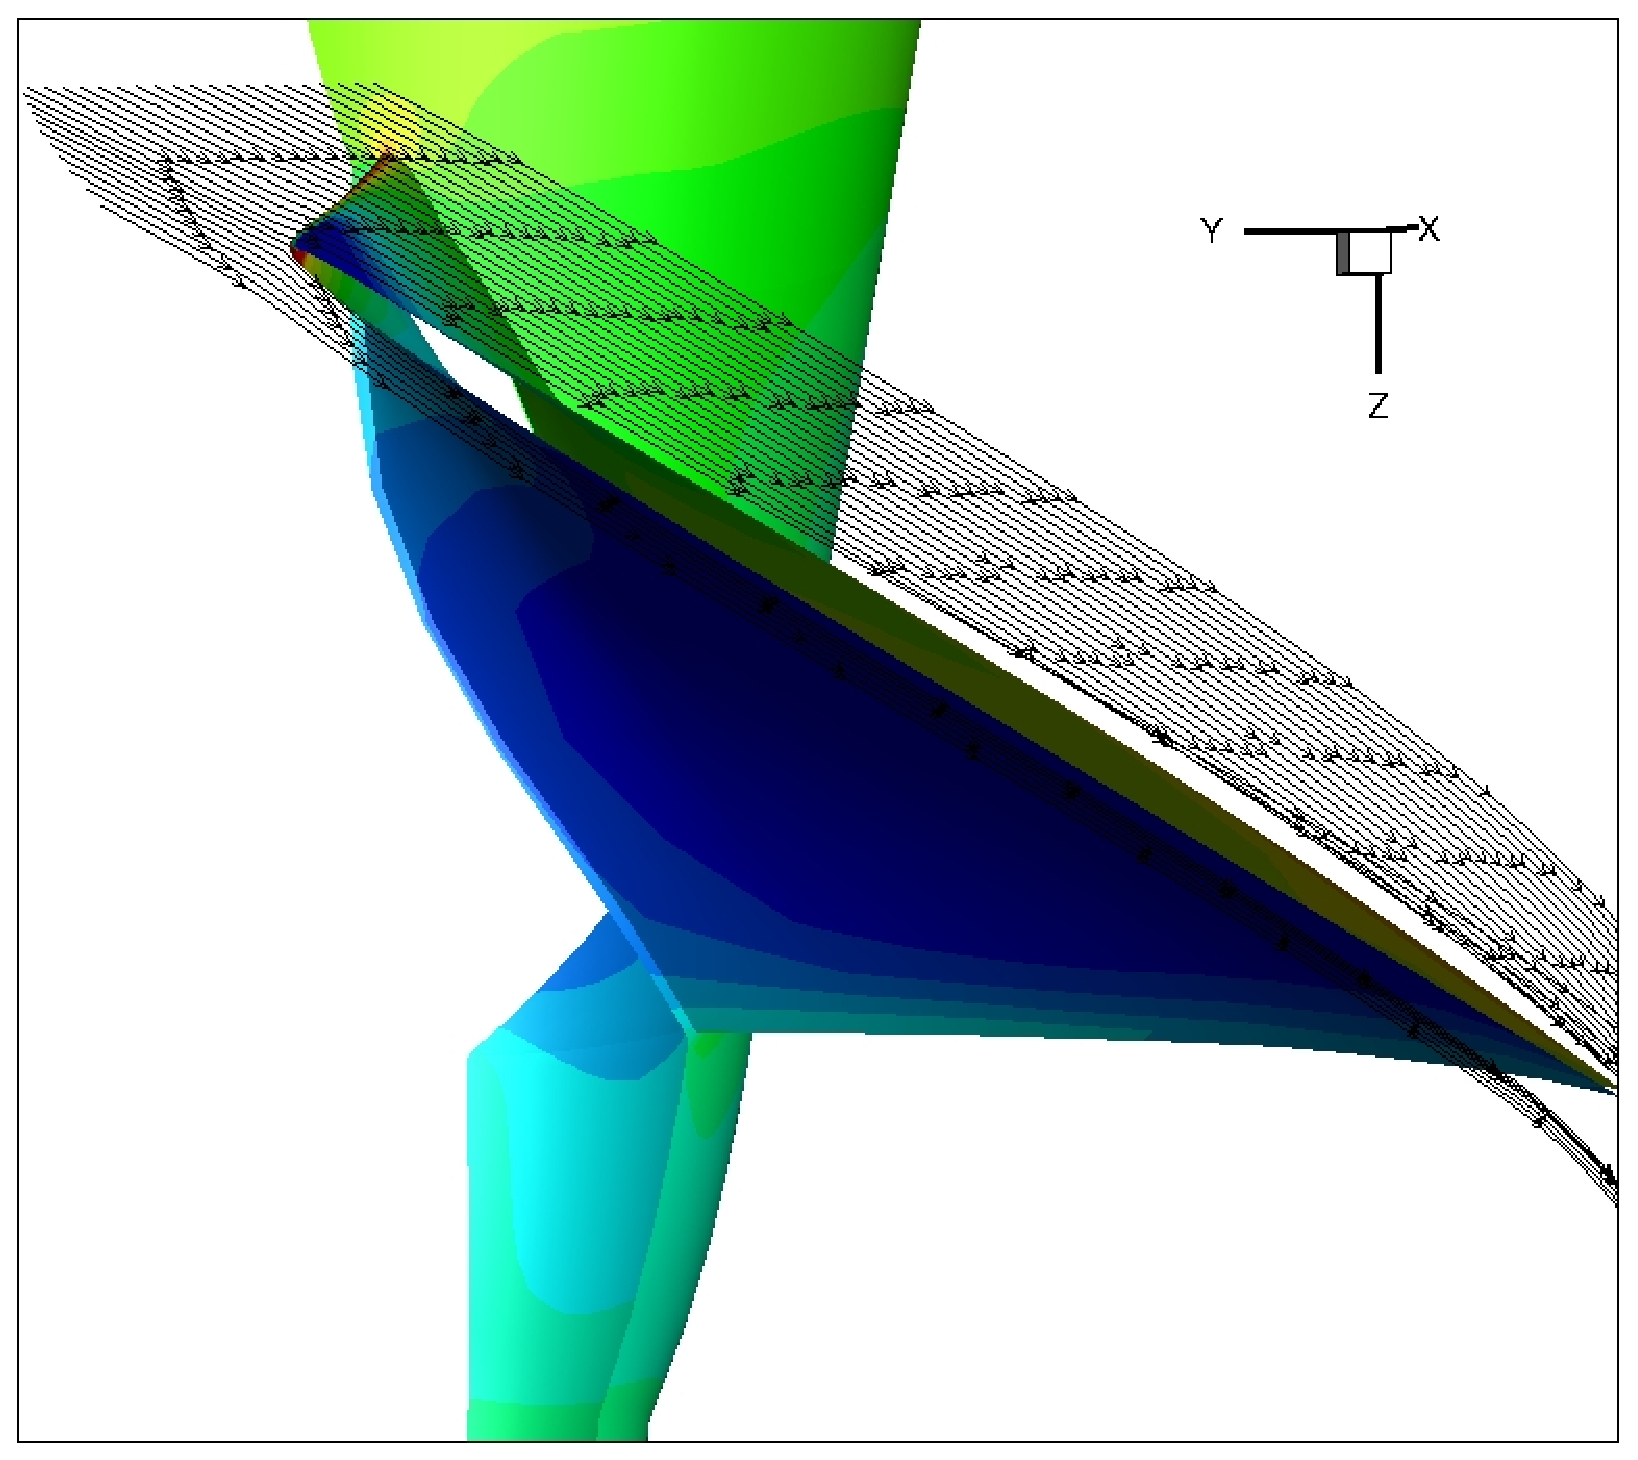
\includegraphics{PartLoad.eps}}
\end{minipage}
\caption{Pressure contour, along with streamlines near the shroud region, at part load operation of a non regulated hydraulic turbine. Water flow near the shroud region meets the blade, for the first time, at the suction side forming the aforementioned pumping surface that needs to be minimized. }
\label{design-pumpS}
\end{figure}

In figure \ref{design-pumpS}, one may observe the flow streamlines, at the near shroud region, and how they meet the blade at the suction side (bottom the this plot). This causes both a high pressure region at the suction side, due to the stagnation point at the point where the flow meets the blade,  and a low pressure region on the pressure side (top here) due to high flow speeds.        

\begin{figure}[h!]
\begin{minipage}[b]{1\linewidth}
 \centering
 \resizebox*{10.0cm}{!}{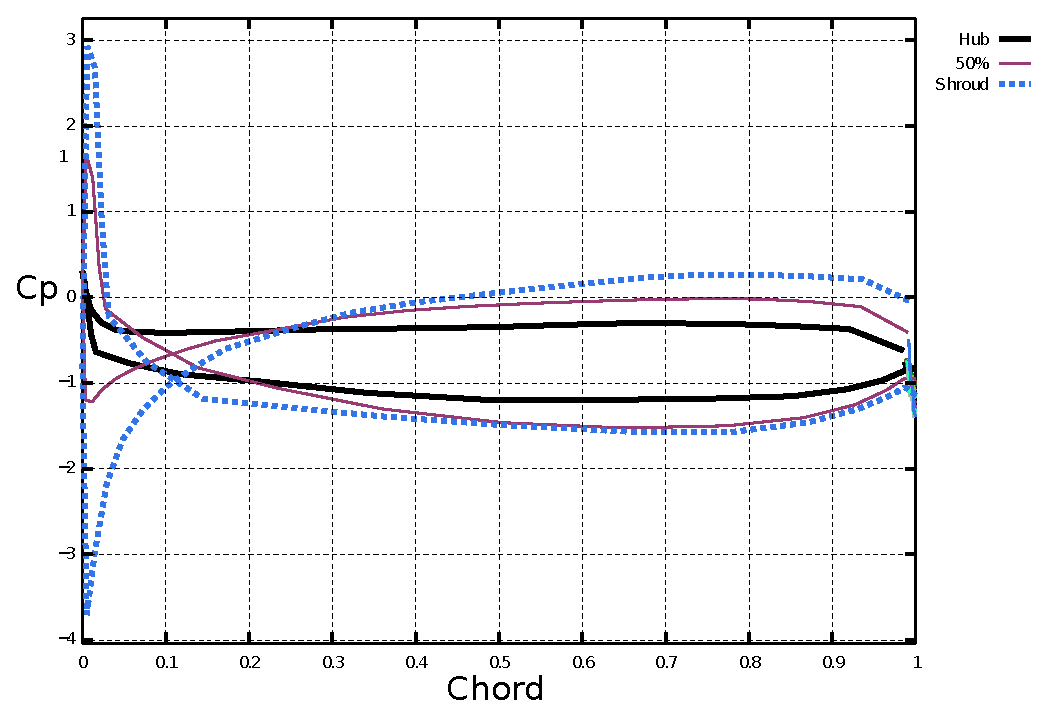
\includegraphics{pumps.eps}}
\end{minipage}
\caption{Pressure coefficient ($C_p$) distribution along the blade chordwise direction at part load operation of a non-regulated hydraulic turbine at three spanwise locations: hub, mid-span and shroud. The pumping area corresponds to the first 10\% of the chord at mid-span and shroud locations}
\label{design-pumpS2}
\end{figure}

The partial pumping operation phenomenon can also be observed by the pressure coefficient ($C_p$) plots, see figure \ref{design-pumpS2}. The near hub $C_p$ distribution (thick continuous line) exhibits no such phenomenon, as expected.  The near shroud $C_p$ distribution (thick dashed line) though suffers from partial pumping operation. The near LE region of the shroud $C_p$ distribution exhibits the so called "crossed" distribution which denotes that the pressure at the pressure side of the blade is lower than that of the suction side. The thin continues line is the mid-span $C_p$ distribution and it also suffers from pumping operation, without however being as severe as close to shroud.        

\section{Optimization of a Francis Turbine} % top level followed by section, subsection
The design/optimization of a Francis turbine runner, in the scope of a modernization/rehabilitation case, will be presented in this section. This case, due to the high number of design variables used to parameterize the candidate geometries, will be used to demonstrate the merits of the KBD method. 
\label{Francis-runner}
\subsection{Francis Turbine}
Francis turbines are the most common water turbine in use today since they can operate in a considerable part of the head-discharge diagram (fig.\ref{range}) \cite{papanto}. Francis is a reaction type water turbine which was named after its developer James B. Francis. 

\begin{figure}[h!]
\centering
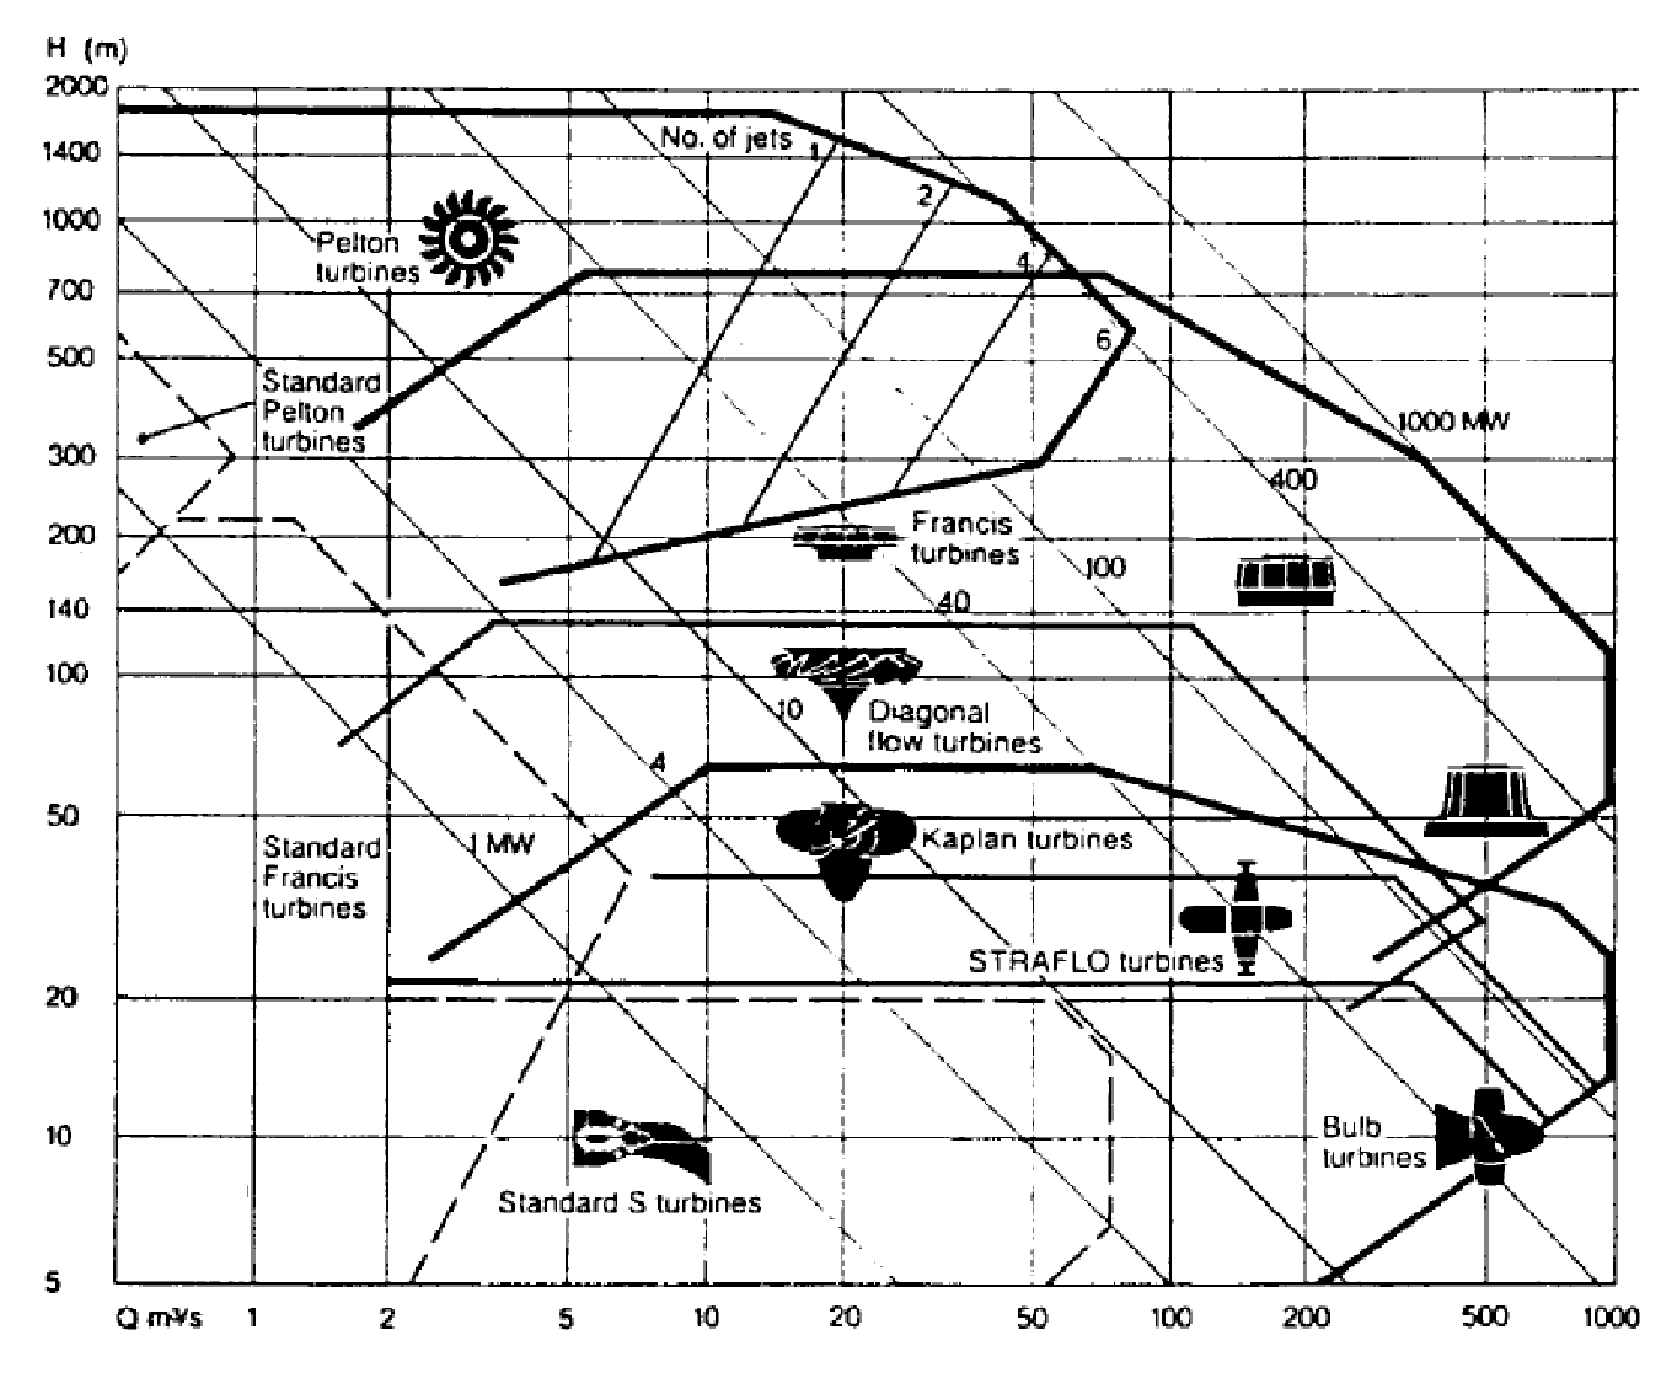
\includegraphics[width=140mm]{range2.eps} 
\caption{Application of different turbine types.}
\label{range}
\end{figure}

A typical Francis turbine consists of four different parts (fig.\ref{francis1}). The Spiral casing  together with the stay-wanes designed to provide uniform water intake around the entire circumference of the wicket-gates inlet. The wicket-gates (or guide-wanes) which are adjustable blades to allow efficient turbine operation for a range of water flow conditions. The runner which is the rotating part harnessing the hydraulic energy. And the draft-tube which is used to control the head of the water working on the turbine via transforming the outlet kinetic energy into head.

\begin{figure}[h!]
\centering
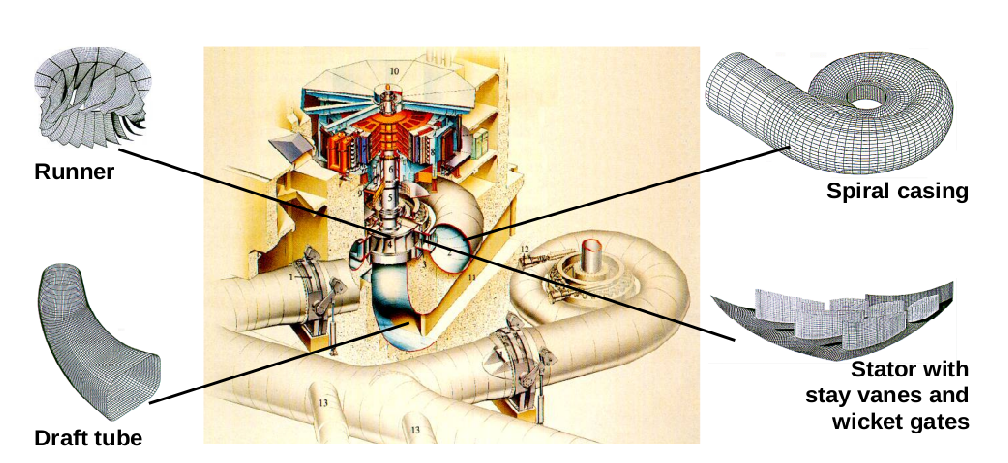
\includegraphics[width=150mm]{francis1.eps} 
\caption{Francis turbine and its consisting parts.}
\label{francis1}
\end{figure}

\subsection{Case presentation}
The design problem in hand is a so-called modernization/rehabilitation project" i.e. upgrade of a runner(fig.\ref{design-parameterization}) in a pre-existing plant. Modernization/rehabilitation projects are fairly common world-wide and specially in Europe where almost all big-hydro locations are already tapped and a lot of them are of a significant age. Typical reasons for modernization/rehabilitation projects are ;
\begin{itemize}
\item reliability and availability increase; 
\item life extension and performance restoration; 
\item performance improvements;
\begin{itemize}
	\item efficiency, power
    \item reduction of cavitation erosion
	\item enlargement of operating range
\end{itemize}
\item plant safety improvement;
\item environmental, social or regulatory issues;
\item maintenance or operating cost reduction;
\item other considerations as
\begin{itemize}
	\item modified governmental regulations
	\item political criteria
	\item modified hydrology conditions
	\item modified market conditions
\end{itemize}
\end{itemize}

In modernization/rehabilitation projects  the designer has to make sure that the newly designed part "runner" has to fit perfectly into the pre-existing structure in respect to both geometry and hydraulic behaviour. Geometry restricts mainly inlet-outlet diameters and hub-shroud meridional contour. Hydraulic behaviour on the other hand enforces given inlet conditions and introduces a new objective, apart from efficiency and cavitation,  witch has to do with drat-tube cabling since the outlet of the newly designed runner is also the draft-tube inlet and any given draft-tube works optimally for a given inlet velocity.      
  
\begin{figure}[h!]
\begin{minipage}[b]{0.5\linewidth}
 \centering
 \resizebox*{4.5cm}{!}{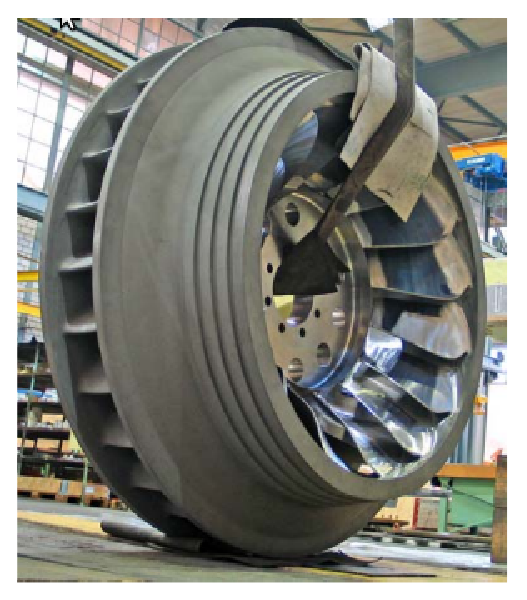
\includegraphics{francis2.eps}}
\end{minipage}
\begin{minipage}[b]{0.5\linewidth}
 \centering
 \resizebox*{7.5cm}{!}{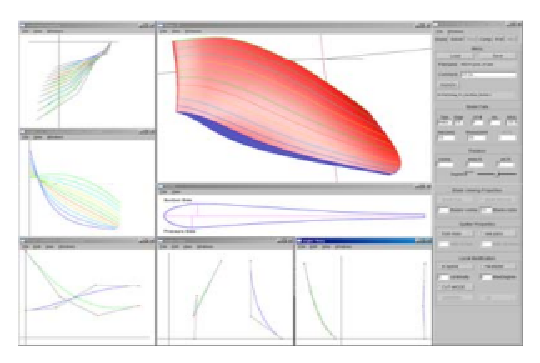
\includegraphics{francis3.eps}}
\end{minipage}
\caption{Optimization of a Francis Turbine: Left; Francic runner. Right; demonstration of Francis runner parameterization}
\label{design-parameterization}
\end{figure}

\subsubsection{Case formulation}
Herein the case formulation that transforms the above design case into a basic optimization problem will be presented. Given that the optimization problem definition is (cite EA chapter);
\begin{align} 
   &min ~ F(x)=(f_1(x),f_1(x),...,f_M(x))\in \Re^{M} \nonumber \\
   &\mbox{subject to} ~ c_k(x)\leq d_k ~ k =1,K
\label{Optim}
\end{align}
,where $x\in X \!\leq\! \Re^{N}$ is the design vector and $X$ the design space, $c(x)$ the constraints vector and $F(x)$ the objectives vector.

\subsubsection{Design parameterization}
The design variables and their corresponding ranges are picked from the set specified in section \ref{Paramt} through a graphical interface integrated in the parameterization tool (fig.\ref{design-parameterization2}).  For the case in hand the design vector consists of $336$ free design variables utilised as follows (table. \ref{design_vars});
\begin{table}[h!]
\begin{center}
\begin{tabular}{ |c|l| }
\hline

Number of              & Design variables determining the:\\
design variables       & \\
\hline
6 & spanwise distributions of $\theta_{LE}$\\
\hline
6 & spanwise distributions of $\theta_{TE}$\\
\hline
6 & spanwise distributions of $\beta_{LE}$\\
\hline
6 & spanwise distributions of $\beta_{TE}$\\
\hline
6 & spanwise distributions of $\zeta_{LE}$\\
\hline
6 & spanwise distributions of $\zeta_{TE}$\\
\hline
6 & spanwise thickness distributions for PS \\
\hline
6 & spanwise thickness distributions for SS\\
\hline
8 & LE meridional position\\
\hline
8 & TE meridional position\\
\hline
4 & Shroud meridional generatrices \\
\hline
4 & Hub meridional generatrices\\
\hline
$12 x 11$ & chordwise thikness destribution for PS (11 profiles)\\
\hline
$12 x 11$ & chordwise thikness destribution for SS (11 profiles)\\
\hline
\hline
336 & Design variables, in total \\
\hline   
\end{tabular}
\caption{
The $336$ design variables used to parameterize the Francis runner.}
\label{design_vars}
\end{center}
\end{table}

\begin{figure}[h!]
\begin{minipage}[b]{0.5\linewidth}
 \centering
 \resizebox*{7.5cm}{!}{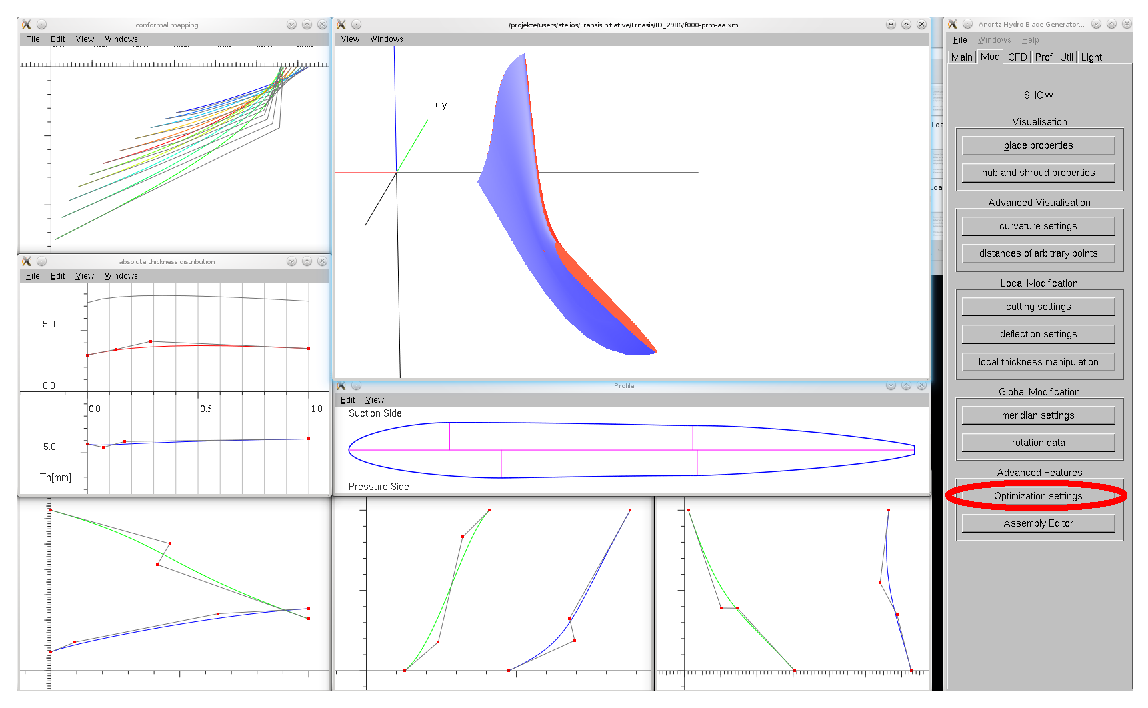
\includegraphics{pic1.eps}}
\end{minipage}
\begin{minipage}[b]{0.5\linewidth}
 \centering
 \resizebox*{7.5cm}{!}{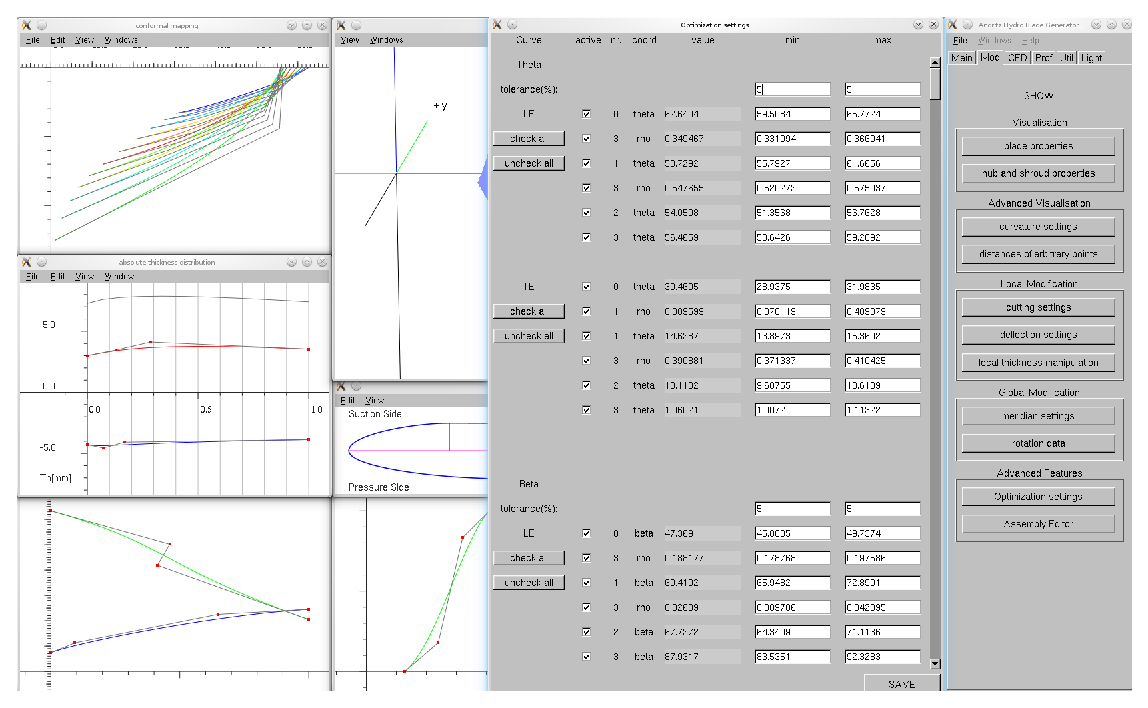
\includegraphics{pic2.eps}}
\end{minipage}
\caption{Optimization of a Francis Turbine: Left; Parameterization tool (optimization settings tab). Right; Francis runner design variable set-up}
\label{design-parameterization2}
\end{figure}

\subsubsection{Objectives \& Constraints}
The objectives vector consist of two objectives, first among them is the outlet velocity profile metric and second is the blade loading quality metric. Loading quality metric minimization is desired, thus creating blades with the biggest possible load uniformity. Outlet velocity profile is also a minimization objective creating blade with the least divergence from the user defined target profiles as they are shown in figure \ref{design-obj-tar}. 

\begin{figure}[h!]
\begin{minipage}[b]{1\linewidth}
 \centering
 \resizebox*{10.0cm}{!}{\includegraphics{Target.eps}}
\end{minipage}
\caption{Optimization of a Francis Turbine: Target undimensional velocity profile distributions.}
\label{design-obj-tar}
\end{figure}


To ensure performance stability, the runner to be designed is desirable to yield optimal performance at three operating points (best efficiency point H=36m, part load H=30m and full load H = 43.5m). The three-operating-point design is handled as an optimization problem with two objectives, where the value of each objective function is computed for each operating point separately and, then, the “overall” value $F_i$ is set equal to the weighted sum of the corresponding values for the three operating points. (table. \ref{op-weights}) 

\begin{table}[h!]
\begin{center}
\begin{tabular}{ |c|l| }
\hline
Operating point& Weigh\\
\hline
best efficiency (BE)  & 1.0\\
\hline
part load (PL) & 0.3\\
\hline
full load (FL) & 0.3\\
\hline
\end{tabular}
\caption{Operating point weights.}
\label{op-weights}
\end{center}
\end{table}


For each of the operating points two constraints are set (table. \ref{Cons}). One to enforce cavitation safety and one to ensure the operating point. Cavitation constraint is based on the $\sigma_{histogram}$ method. Operating point control is materialised with a constrain that is defined as a maximum distance from the desired operating point (fig.\ref{design-obj3}). Depending on the solver set-up this could be either the massflow or the Hydraulic height.     


\begin{table}[h!]
\begin{center}
\begin{tabular}{ |c|c|c| }
\hline
Operating point & $\sigma = -\sigma_i^{Hist}$ & Operating point distance\\
\hline
BE & $> -0.2$ & $<1.5\%$\\
\hline
PL       & $> -0.2$ & $<5\%$\\
\hline
FL       & $> -0.2$ & $<5\%$\\
\hline
\end{tabular}
\caption{Constraints per operating point.}
\label{Cons}
\end{center}
\end{table}


\begin{figure}[h!]
%\begin{minipage}[b]{0.5\linewidth}
% \centering
% \resizebox*{7.0cm}{!}{\includegraphics{sigma.eps}}
%\end{minipage}
\begin{minipage}[b]{1\linewidth}
 \centering
 \resizebox*{10.0cm}{!}{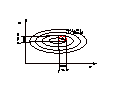
\includegraphics{con1.eps}}
\end{minipage}
\caption{Optimization of a Francis Turbine: Maximum distance from operating point equals to $\pm2\%$.}
\label{design-obj3}
\end{figure}

\subsection{Results}
As mention above this case is used to demonstrate the merits of the first original idea proposed in this thesis namely the KBD method in a real industrial case. Therefore two optimizations will take place; One utilizing the traditional EA since the large number of design varibles ($336$) deems the use of MAEA non productive; And one utilizing the MAEA(KBD) method.

\subsubsection{Archived designs}
 Three archived designs where available (fig. \ref{design-bases}). This designs were developed to perform optimally in neighbouring operating points to the desired blade. The criteria used to estimate this vicinity were the undimensional specific speed $N_{ED}$ and specific massflow $Q_{ED}$. Since this design were fitted with their own, power plan specific, hub and shroud contours and given that during the modernization/rehabilitation project in hand this contours was asked to remain similar to the initial blade, some modifications were required in order to transform the archived designs into compatible with the required hub and shroud contours limitations. This modification were restricted to simple stretching and cutting something that requires practically zero time for the designer. However, as will be shown later in this section, this leads to altered designs with questionable quality. Nevertheless this designs, with out any further hand-made refinements, are sufficient to be used as basis vectors in the KBD method.                           

\begin{figure}[h!]
\begin{minipage}[b]{1\linewidth}
 \centering
 \resizebox*{10.0cm}{!}{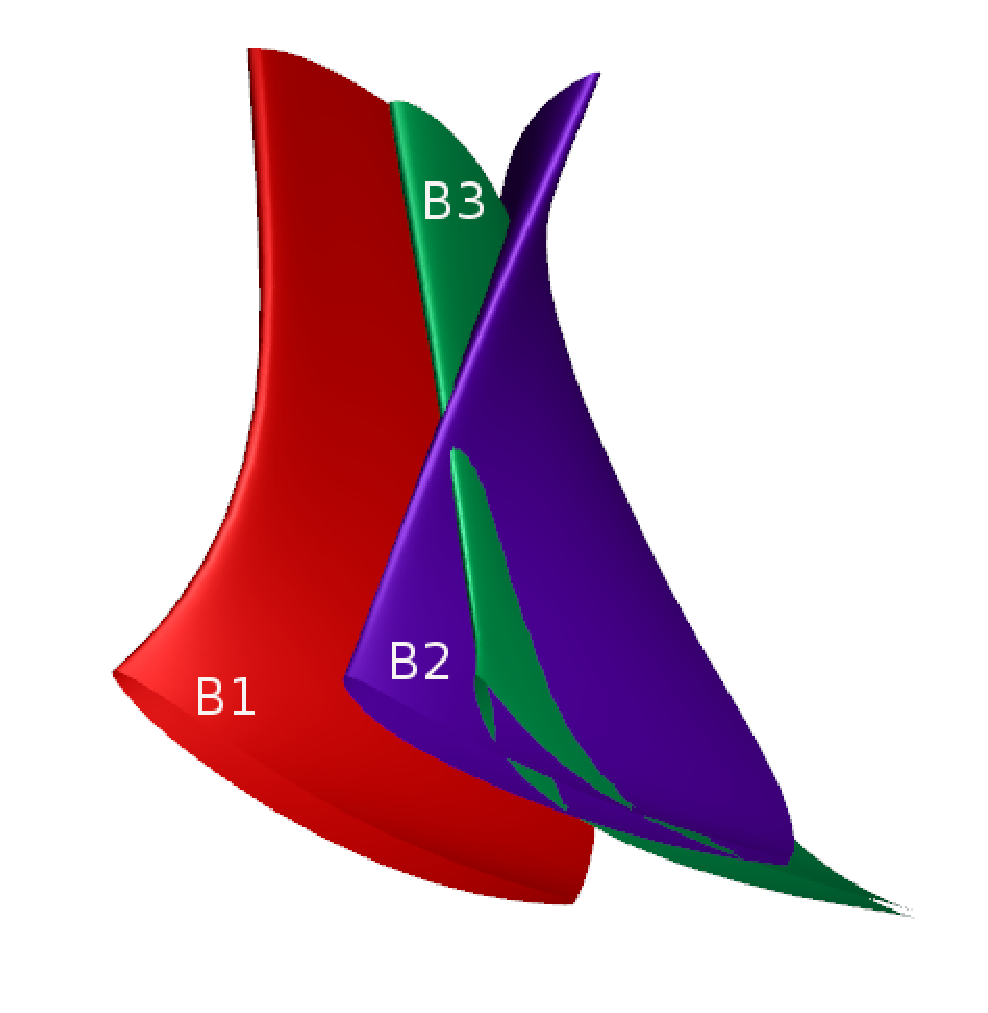
\includegraphics{Francis_bases.eps}}
\end{minipage}
\caption{Optimization of a Francis Turbine: The three archived geometries used for this case.}
\label{design-bases}
\end{figure}

The archived designs to be used as basis vectors for this case are re-evaluated at the desirable operating points and their quality metrics are summarized in table \ref{reuse}.

\begin{table}[h!]
\begin{center}
\begin{tabular}{ |c|c|c|c|c|c| }
\hline
Geometry & OP & Outlet quality & Blade loading  & Cavitation & H\\
\hline
B1 & BE & $0.472$ & $0.538$ & $-0.21 < -0.2$ ! & $ 5\% >1.5\%$ ! \\
B1 & PL & $0.552$ & $0.824$ & $-0.23 < -0.2$ ! & $ 3.6\% <5\%$ \\
B1 & FL & $0.408$ & $0.594$ & $-0.2 = -0.2$  & $ 5.7\% >5\%$ ! \\
\hline
\hline
B2 & BE & $0.563$ & $0.922$ & $-0.22 < -0.2$ ! & $ 3.8\% >1.5\%$ ! \\
B2 & PL & $0.534$ & $0.888$ & $-0.24 < -0.2$ ! & $ 2.6\% <5\%$  \\
B2 & FL & $0.522$ & $1.178$ & $-0.22 < -0.2$ ! & $ 4.8\% <5\%$  \\
\hline
\hline
B3 & BE & $0.402$ & $0.663$ & $-0.19 > -0.2$  & $ 6.8\% >1.5\%$ ! \\
B3 & PL & $0.515$ & $0.808$ & $-0.21 < -0.2$ ! & $ 6.9\% >5\%$ ! \\
B3 & FL & $0.257$ & $0.896$ & $-0.18 > -0.2$  & $ 7.1\% >5\%$ ! \\
\hline
\end{tabular}
\caption{Quality metrics (objectives and constraints) for the 3 archived designs (B1,B2 $\&$ B3) for all operating points (BE,PL $\&$ FL). Explanation mark next to an inequality means that the related constrained is violated}
\label{reuse}
\end{center}
\end{table}

A closer look on B1 reviles the summarized in table \ref{reuse} findings. Firstly, figure \ref{Francis-B1-BE} the $\sigma$ contour is plotted ove the runner surfaces. In this figure one may observe the lower limit of $\sigma = -0.216$ which advocates the presence of cavitation even for the BE operating point. Cavitation is observed at suction side near the trailing edge between mid-span and shroud. Archived design B1 suffers from cavitation also for PL operating point and is marginally safe for FL (table \ref{reuse}). 

\begin{figure}[h!]
\begin{minipage}[b]{1\linewidth}
 \centering
 \resizebox*{11.0cm}{!}{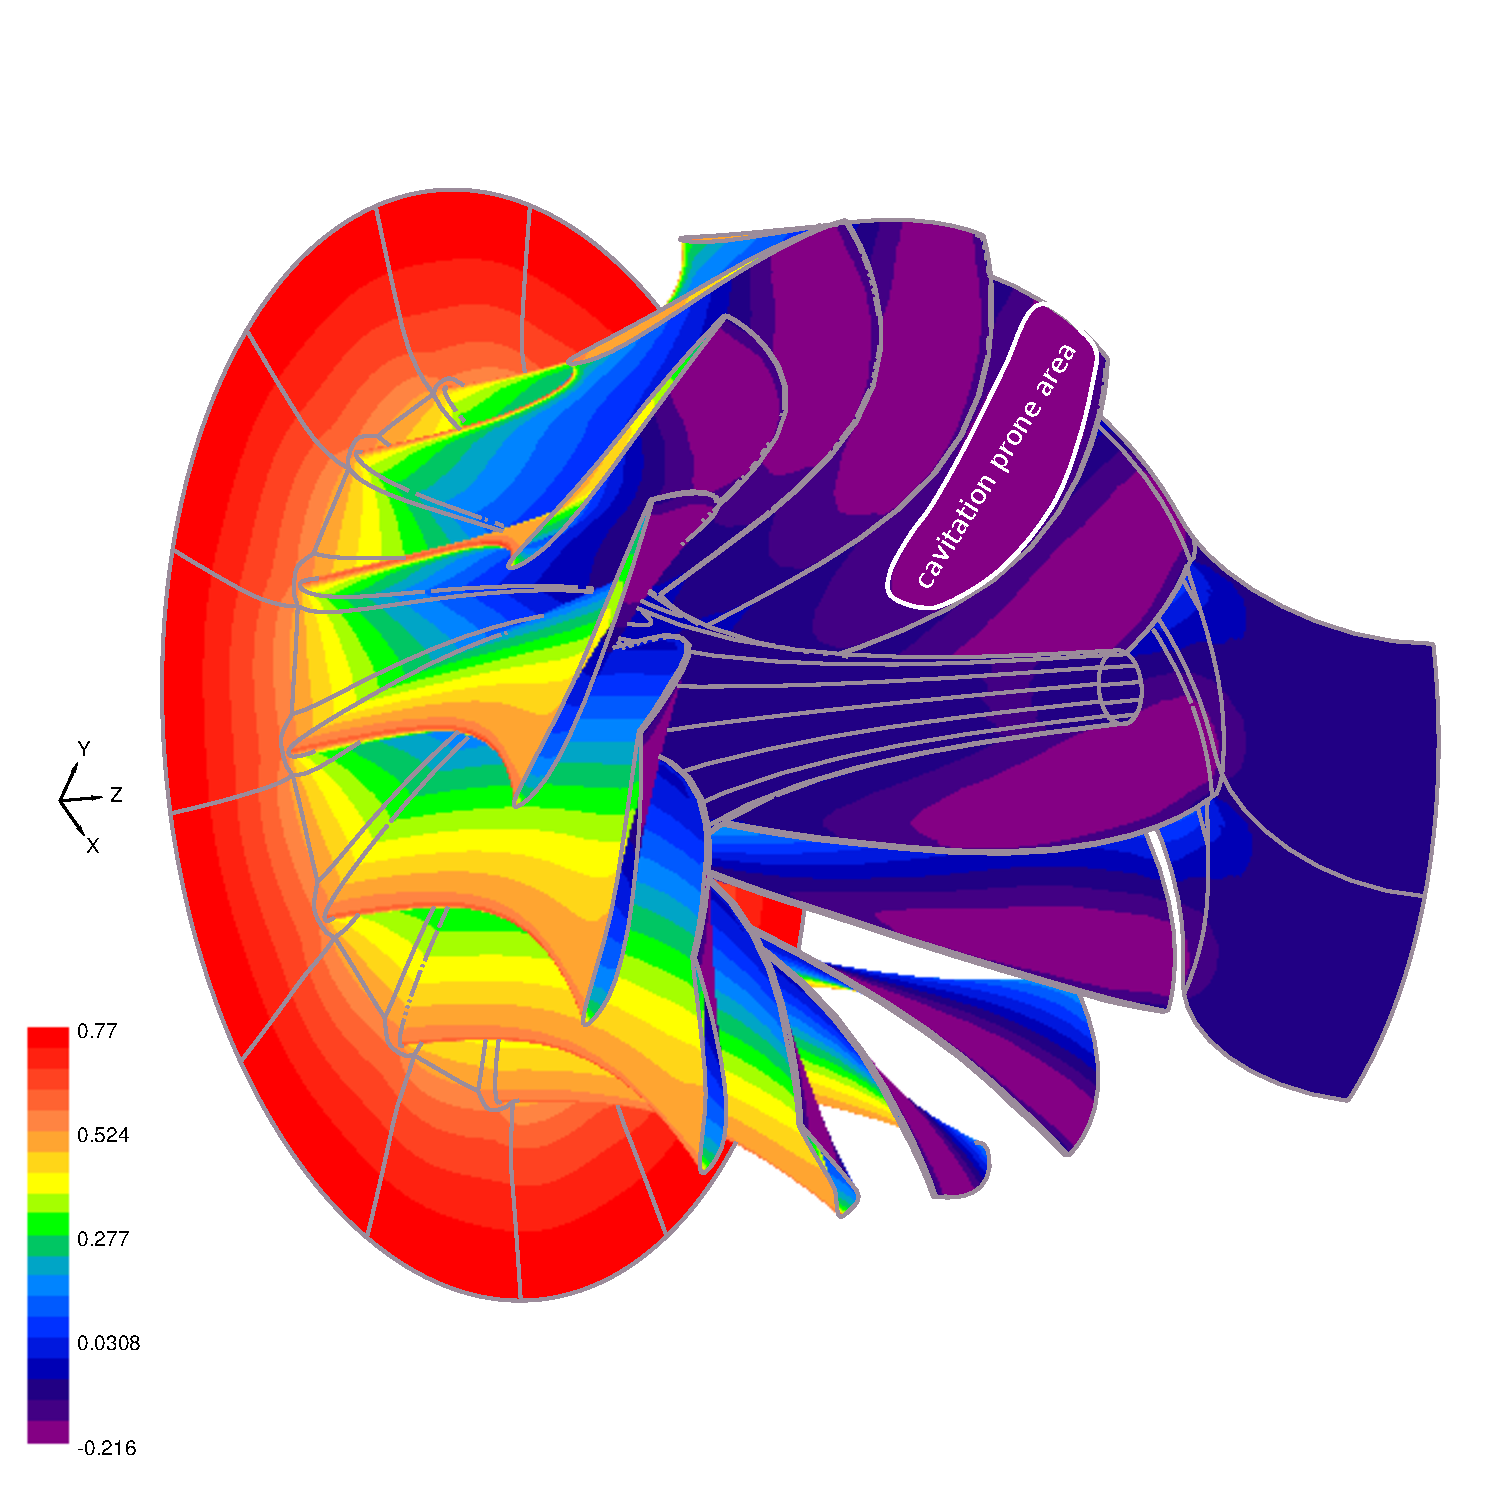
\includegraphics{B1.eps}}
\end{minipage}
\caption{Optimization of a Francis Turbine: $\sigma$ contour for archived geometry B1 at BE operating point.}
\label{Francis-B1-BE}
\end{figure}

Furthermore, in figure \ref{Francis-B1-OUT} one can observe the big deviation from the desirable outlet $C_m$ and $C_u$ velocity components for the BE operating point.  Dashed lines represent $C_m$ and continues lines $C_u$. For purpose of comparison in the same plot the target distributions are plotted with thicker lines.   

\begin{figure}[h!]
\begin{minipage}[b]{1\linewidth}
 \centering
 \resizebox*{9.0cm}{!}{\includegraphics{OUTLET_B1.eps}}
\end{minipage}
\caption{Optimization of a Francis Turbine: $C_m$ and $C_u$ profiles for archived geometry B1 at BE operating point.}
\label{Francis-B1-OUT}
\end{figure}

The loading quality can be demonstrated through the chord-wise $C_p$ (eq. \ref{Cpdef}) distribution along the hub, shroud and mid-span positions (fig. \ref{Francis-B1-LOAD}). Although mid-span and hub demonstrate relatively good loading behaviour shroud position suffers for big load differences.      

\begin{figure}[h!]
\begin{minipage}[b]{1\linewidth}
 \centering
 \resizebox*{9.0cm}{!}{\includegraphics{Load_B1.eps}}
\end{minipage}
\caption{Optimization of a Francis Turbine: $C_p$ profiles hub, mid-span and shroud for archived geometry B1 at BE operating point.}
\label{Francis-B1-LOAD}
\end{figure}

Regarding B2, the geometry suffers from cavitation in all operating points BE,PL and FL as it is illustrated in table \ref{reuse}. Figure \ref{Francis-B2-BE} depicts the $\sigma$ contour concerning the archived geometry B2. The lower limit of $\sigma = -2.34$ which denoted the presence of cavitation. Cavitation is observed at suction side near the trailing edge at the near hub region.     


\begin{figure}[h!]
\begin{minipage}[b]{1\linewidth}
 \centering
 \resizebox*{11.0cm}{!}{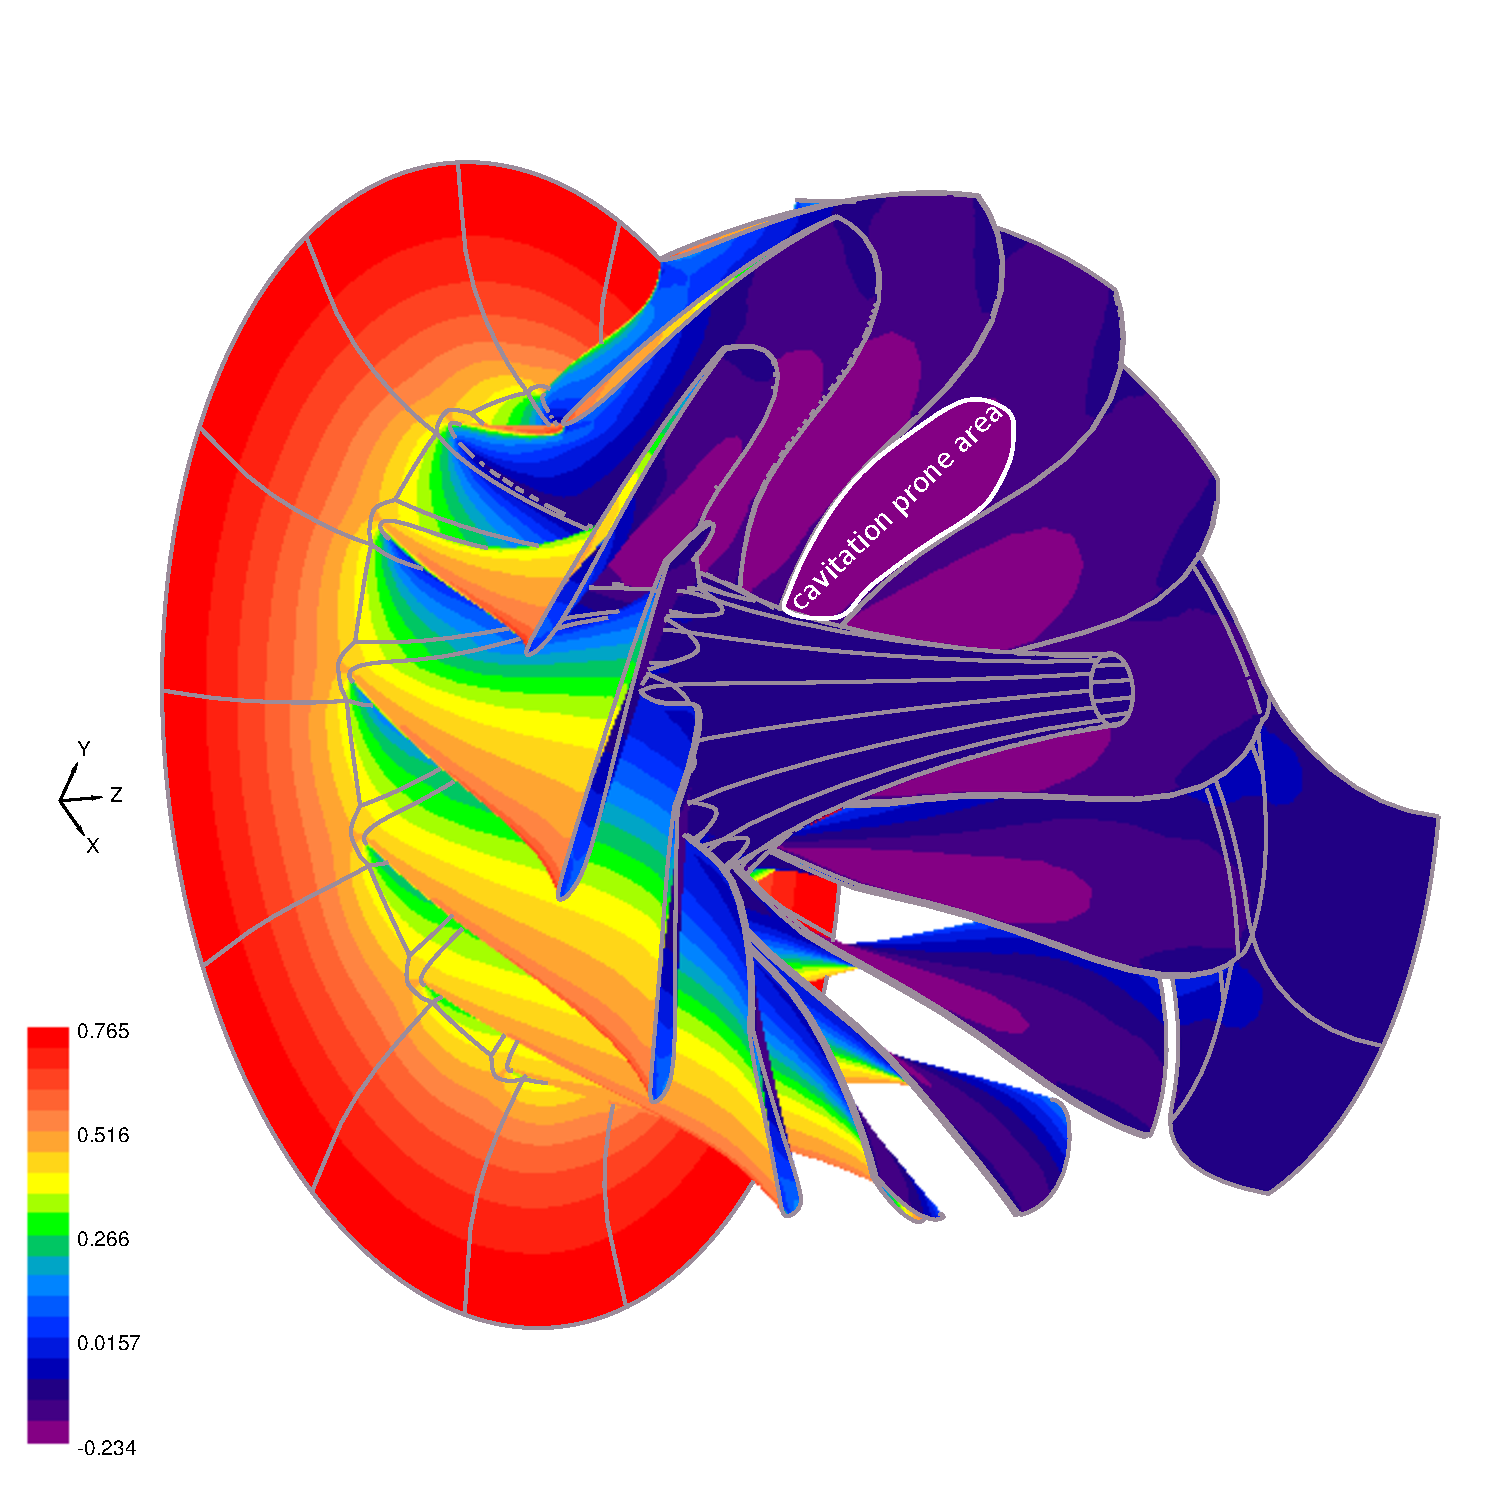
\includegraphics{B2.eps}}
\end{minipage}
\caption{Optimization of a Francis Turbine: $\sigma$ contour for archived geometry B2 at BE operating point.}
\label{Francis-B2-BE}
\end{figure}

Outlet velocity quality is demonstrated in figure \ref{Francis-B2-OUT}. $C_m$ is fur away from the desirable distribution and $C_u$ has high values at the near hub region.   

\begin{figure}[h!]
\begin{minipage}[b]{1\linewidth}
 \centering
 \resizebox*{9.0cm}{!}{\includegraphics{OUTLET_B2.eps}}
\end{minipage}
\caption{Optimization of a Francis Turbine: $C_m$ and $C_u$ profiles for archived geometry B2 at BE operating point.}
\label{Francis-B2-OUT}
\end{figure}

Observing the $C_p$ profiles for archived geometry B2 for the BE operating point (fig. \ref{Francis-B2-LOAD}) one can observe the bud loading quality, as it is depicted also in table \ref{reuse}. For all three positions there are big load differences along the chord direction (from LE to TE). 

\begin{figure}[h!]
\begin{minipage}[b]{1\linewidth}
 \centering
 \resizebox*{9.0cm}{!}{\includegraphics{Load_B2.eps}}
\end{minipage}
\caption{Optimization of a Francis Turbine: $C_p$ profiles hub, mid-span and shroud for archived geometry B2 at BE operating point.}
\label{Francis-B2-LOAD}
\end{figure}

Archived geometry B3 is clean from cavitation in all but PL operating point as it is illustrated in table \ref{reuse}. Figure \ref{Francis-B3-PL} depicts the $\sigma$ contour concerning the archived geometry B3 for the crucial PL operating point. The lower limit of $\sigma = -2.15$ shows the presence of cavitation. Cavitation is observed at suction side near the trailing edge.     


\begin{figure}[h!]
\begin{minipage}[b]{1\linewidth}
 \centering
 \resizebox*{11.0cm}{!}{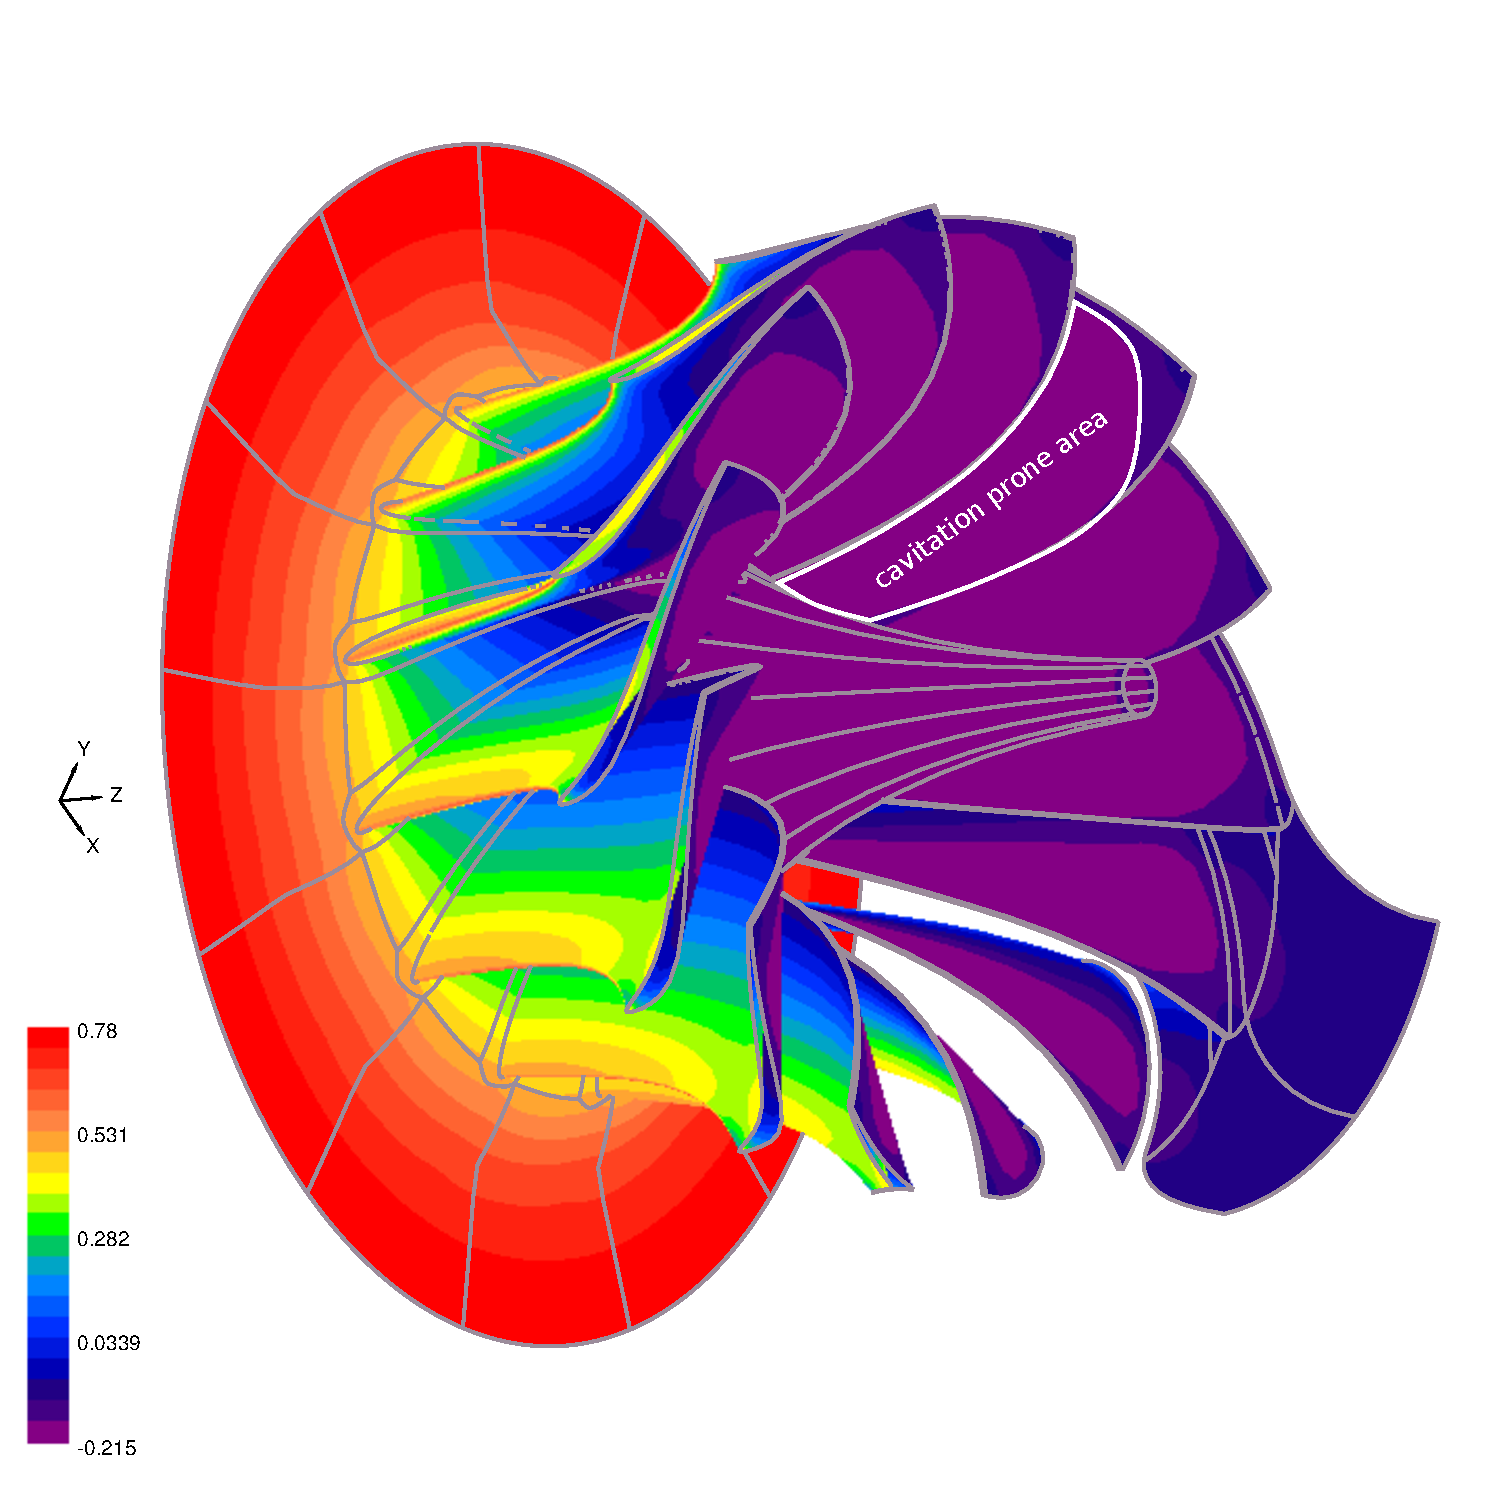
\includegraphics{B3.eps}}
\end{minipage}
\caption{Optimization of a Francis Turbine: $\sigma$ contour for archived geometry B3 at PL operating point.}
\label{Francis-B3-PL}
\end{figure}

Regarding the outlet velocity quality, see figure \ref{Francis-B3-OUT}, both $C_m$  and $C_u$ are away form the desirable distributions.   

\begin{figure}[h!]
\begin{minipage}[b]{1\linewidth}
 \centering
 \resizebox*{9.0cm}{!}{\includegraphics{OUTLET_B3.eps}}
\end{minipage}
\caption{Optimization of a Francis Turbine: $C_m$ and $C_u$ profiles for archived geometry B3 at BE operating point.}
\label{Francis-B3-OUT}
\end{figure}

Loading quality is demonstrated in figure \ref{Francis-B3-LOAD}). The $C_p$ profile at the shroud position reviles big loading differences. 

\begin{figure}[h!]
\begin{minipage}[b]{1\linewidth}
 \centering
 \resizebox*{9.0cm}{!}{\includegraphics{Load_B3.eps}}
\end{minipage}
\caption{Optimization of a Francis Turbine: $C_p$ profiles hub, mid-span and shroud for archived geometry B3 at BE operating point.}
\label{Francis-B3-LOAD}
\end{figure}

The fact that neither of the three archived designs neither shows good outlet and loading qualities nor respects the enforced constraints reveals the necessity of a revise step. The revise step takes place using an EA as a design/optimization technique. Two separate optimization procedure will take place in order to demonstrate the merits of the proposed in this PhD thesis KBD method. One will use a traditional EA ($\mu=30,\lambda=120$) using the $336$ design variables, the use of metamodels in such a high dimensional space is deemed non profitable. The second optimization procedure will use the proposed KBD method, MAEA(KBD) ($\mu=20,\lambda=60,\lambda_e= 4 ~ to~ 8$, ipe phase starting after $150$ non-failed individuals in the DB) , with $19$ optimization variables. For both of the optimizations the three archived designs are injected in the first EA generation.

The $19$ optimization variables are generated (eq. \ref{non-linear2}) from the grouping of the design variables of each archived geometries into $6$ groups (table \ref{design_groups}) and the introduction of the extrapolation variable $\Phi$. This arrangement generated $6$ weights controlling the influence of each archived geometry for the candidate solution thus $18$ weight in total. The $18$ weights plus the extrapolation variable $\Psi$ are the $19$ optimization variables.         


\begin{table}[h!]
\begin{center}
\begin{tabular}{ |c|l| }
\hline

Group              & Design variables determining the:\\
\hline
1 & spanwise distributions of $\theta_{LE}$\\
\hline
1 & spanwise distributions of $\theta_{TE}$\\
\hline
2 & spanwise distributions of $\beta_{LE}$\\
\hline
2 & spanwise distributions of $\beta_{TE}$\\
\hline
3 & spanwise distributions of $\zeta_{LE}$\\
\hline
3 & spanwise distributions of $\zeta_{TE}$\\
\hline
4 & spanwise thickness distributions for PS \\
\hline
4 & spanwise thickness distributions for SS\\
\hline
5 & LE meridional position\\
\hline
5 & TE meridional position\\
\hline
5 & Shroud meridional generatrices \\
\hline
5 & Hub meridional generatrices\\
\hline
6 & chordwise thikness destribution for PS (11 profiles)\\
\hline
6 & chordwise thikness destribution for SS (11 profiles)\\
\hline
\hline
6 & Groups, in total \\
\hline   
\end{tabular}
\caption{
The $6$ Groups used to form the optimization variables as proposed by the KBD method.}
\label{design_groups}
\end{center}
\end{table}

The convergence comparison between EA and MAEA(KBD) is demonstrated using the hyper-volume indicator \cite{Zitz2007}. The Hyper-volume indicator assumes that the quality of a Pareto front can be quantified in a scalar value that is the dominated, by the Pareto front, portion of the objective space as it is restricted by a constant reference point.  The larger value the hyper-volume indicator has the grated is the quality of the Pareto front in hand is.

The Hyper-volume indicators versus the exact evaluations performed of the two optimization procedures are depicted in figure \ref{Francis-Res}. The exact evaluation count is used as a measure of the computational cost.     


\begin{figure}[h!]
\begin{minipage}[b]{1\linewidth}
 \centering
 \resizebox*{10.0cm}{!}{\includegraphics{HypComp.eps}}
\end{minipage}
\caption{Optimization of a Francis Turbine: Hyper-volume comparison between EA and the proposed MAEA(KBD) method.}
\label{Francis-Res}
\end{figure}

The MAEA(KBD) method significantly outperforms the classic EA. It starts with a significantly better prediction for the first generation something that demonstrates that, even though the  archived geometries are not even close to the optimal design, the grouping of the design variables and the incorporation of normal distribution in order to set importance regions in the design space are very close to the problem physics.    

\begin{figure}[h!]
\begin{minipage}[b]{1\linewidth}
 \centering
 \resizebox*{10.0cm}{!}{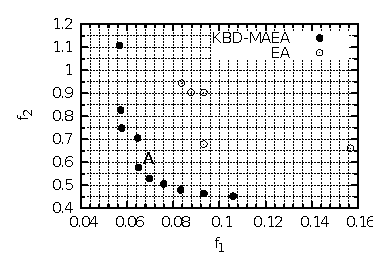
\includegraphics{Comp.eps}}
\end{minipage}
\caption{Optimization of a Francis Turbine: Fronts of non-dominated solutions as they are aquaried for the cost of $1500$ exact evaluations for the EA and MAEA(KBD) method. The decision maker, design engineer, finally chose design A as the most appropriate one among the non dominated members of the Pareto front.}
\label{Francis-Res-par}
\end{figure}

Looking at the final pareto fronts of the two methods (fig. \ref{Francis-Res-par}), for the same computational cost of $1500$ exact evaluations, the increased quality of the designs acquired by the MAEA(KBD) method is evident. Finally the decision maker, design engineer, has choose among the non-dominated members of the final Pareto front design A (fig.\ref{design-bases-a}) as the design that incorporates the best compromise between the two objectives.


\begin{figure}[h!]
\begin{minipage}[b]{1\linewidth}
 \centering
 \resizebox*{10.0cm}{!}{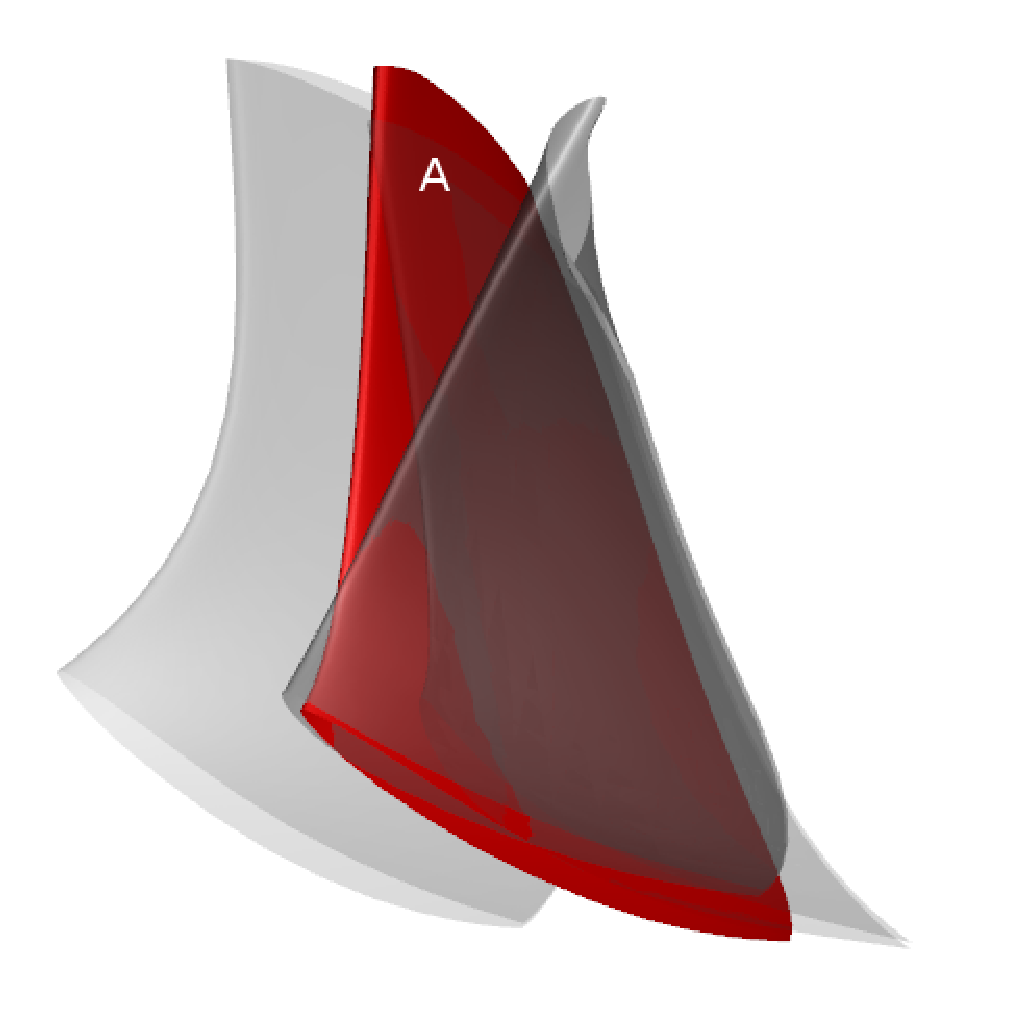
\includegraphics{final.eps}}
\end{minipage}
\caption{Optimization of a Francis Turbine: Design A and the three archived geometries used for this case.}
\label{design-bases-a}
\end{figure}

The quality metric of design A are summarized in table \ref{Asum}. This metrics should be compared with the values in table \ref{reuse}. Design A is significantly better that the three archived designs at all operating points and for both objectives. Design A is an overall high quality blade.


\begin{table}[h!]
\begin{center}
\begin{tabular}{ |c|c|c|c|c|c| }
\hline
Geometry & OP & Outlet quality & Blade loading  & Cavitation & H\\
\hline
A & BE & $0.001$ & $0.302$ & $-0.18 > -0.2$ & $ 1.1\% <1.5\%$ \\
A & PL & $0.086$ & $0.409$ & $-0.19 > -0.2$ & $ 1.5\% <5\%$ \\
A & FL & $0.092$ & $0.504$ & $-0.18 > -0.2$ & $ 4.1\% <5\%$  \\
\hline
\end{tabular}
\caption{Quality metrics (objectives and constraints) regarding the chosen design A for all operating points (BE,PL $\&$ FL). The design is safe from cavitation for all operating points and it operates within the desirable operation range.}
\label{Asum}
\end{center}
\end{table} 

Cavitational behaviour of the selected design A is, in a more detailed manner, observable in figures \ref{Francis-A-BE}, \ref{Francis-A-PL} and \ref{Francis-A-FL} regarding BE,PL and FL operating points respectively.      


\begin{figure}[h!]
\begin{minipage}[b]{1\linewidth}
 \centering
 \resizebox*{11.0cm}{!}{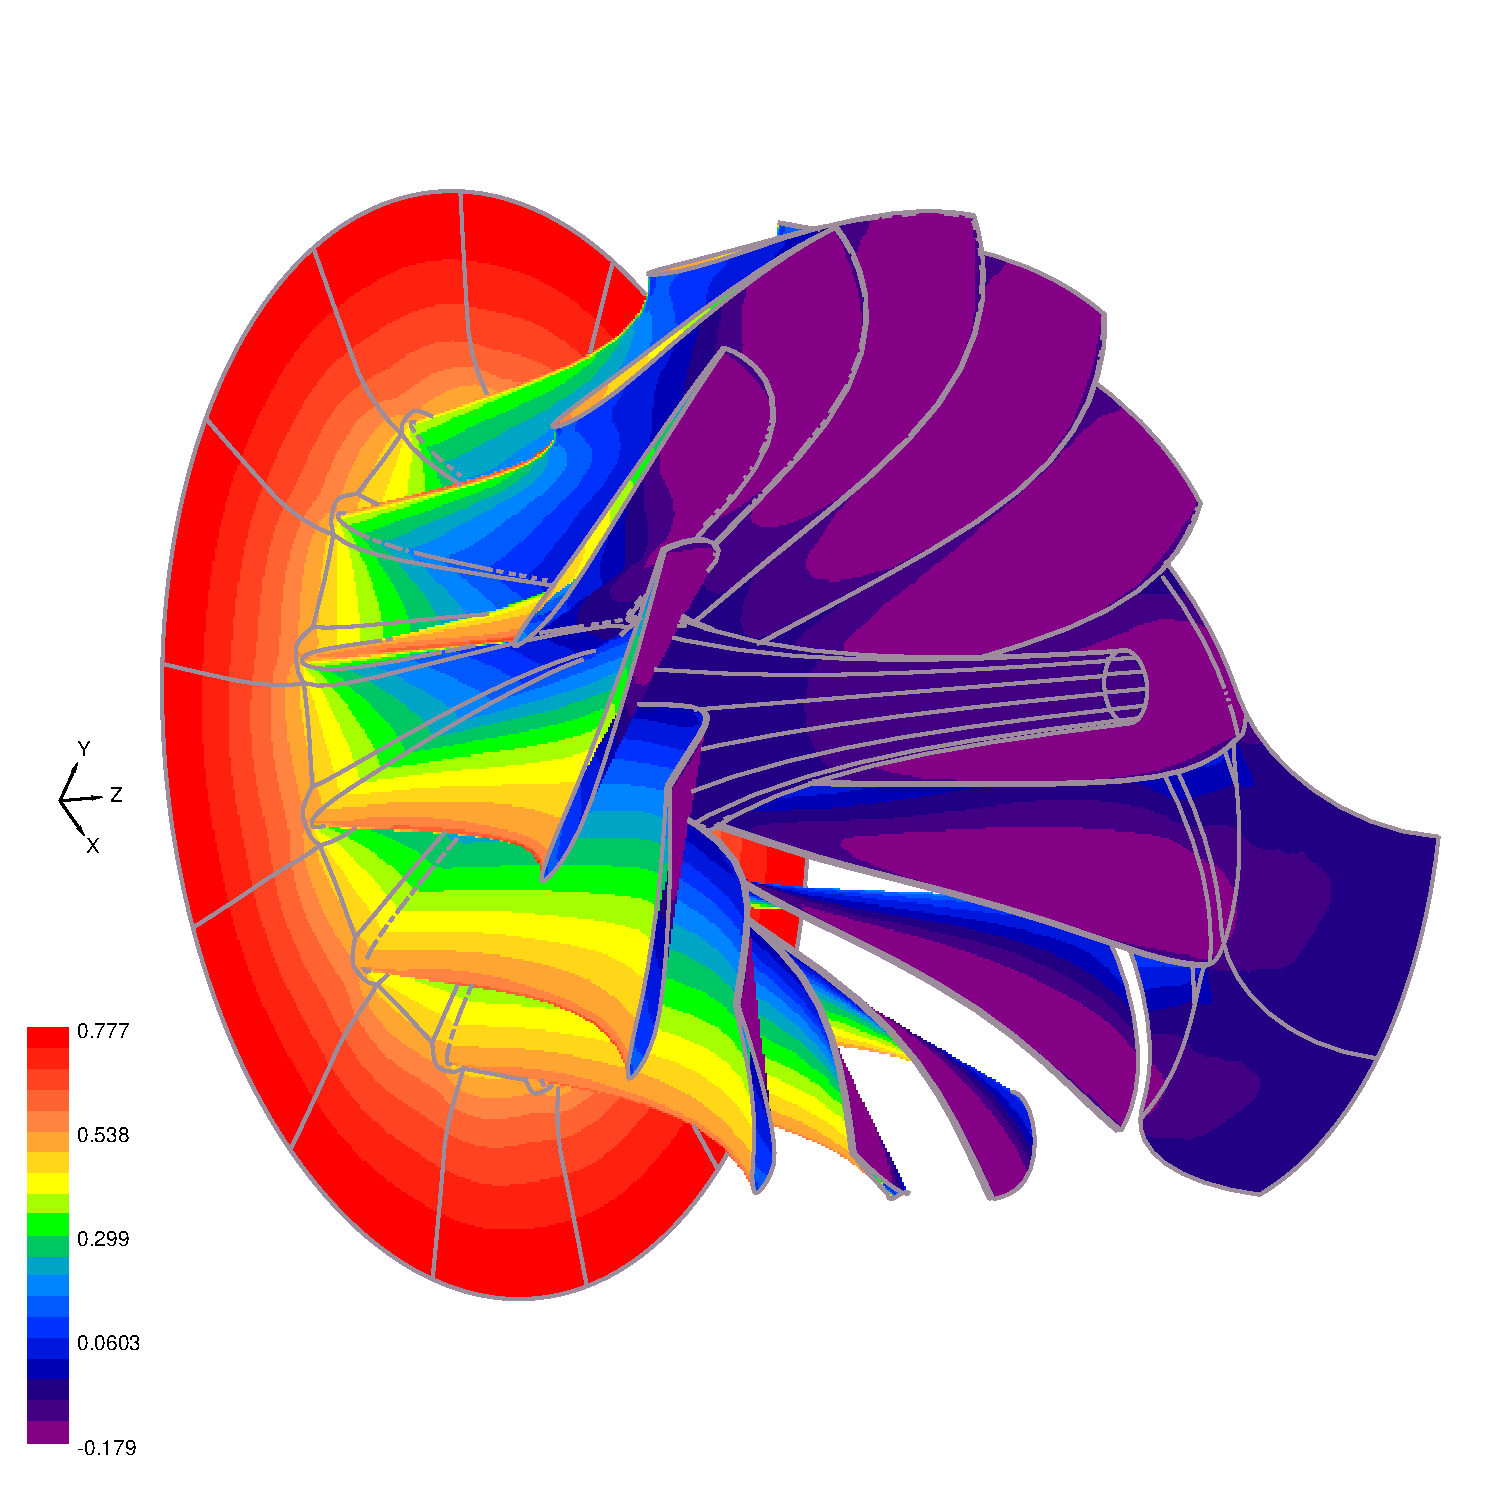
\includegraphics{ABE.eps}}
\end{minipage}
\caption{Optimization of a Francis Turbine: $\sigma$ contour for design A at BE operating point.}
\label{Francis-A-BE}
\end{figure}

Regarding the BE operating point the lowest observable $\sigma$ value is $-0.179$ well above the $-0.2$ desirable limit. 

\begin{figure}[h!]
\begin{minipage}[b]{1\linewidth}
 \centering
 \resizebox*{11.0cm}{!}{\includegraphics{APL.eps}}
\end{minipage}
\caption{Optimization of a Francis Turbine: $\sigma$ contour for design A at PL operating point.}
\label{Francis-A-PL}
\end{figure}

For PL operating point the lowest $\sigma$ value is equal to $-0.192$ which closer to the $-0.2$ limit but still safe. Typically off-design points, such as PL and FL, operate closer to the cavitation danger zone. Design A when operating at PL demonstrates the lower values of $\sigma$ at the suction side of the blade near the leading edge as it is shown in figure \ref{Francis-A-PL}.  
 

\begin{figure}[h!]
\begin{minipage}[b]{1\linewidth}
 \centering
 \resizebox*{11.0cm}{!}{\includegraphics{AFL.eps}}
\end{minipage}
\caption{Optimization of a Francis Turbine: $\sigma$ contour for design A at FL operating point over suction side.}
\label{Francis-A-FL}
\end{figure}

Regarding FL operating point, the lowest observable $\sigma$ value is $-0.182$ (fig. \ref{Francis-A-FL}) also closer to the limit than the BE operating point as expected. Operating at FL design A demonstrates the lower $\sigma$ values, apart form the trailing edge, also near the leading edge at suction side (fig. \ref{Francis-A-SS}). 


\begin{figure}[h!]
\begin{minipage}[b]{1\linewidth}
 \centering
 \resizebox*{9.0cm}{!}{\includegraphics{ASS.eps}}
\end{minipage}
\caption{Optimization of a Francis Turbine: $\sigma$ contour for design A at FL operating point.}
\label{Francis-A-SS}
\end{figure}

Furthermore the outlet quality of design A at BE operating point is demonstrated in figure  \ref{Francis-A-OUT}. Design A clearly outperforms all three archived designs regarding the outlet quality metric. A very close match with the desirable distributions is achieved, in fact according to expert design engineers this amount of divergence is in reality negligible.

\begin{figure}[h!]
\begin{minipage}[b]{1\linewidth}
 \centering
 \resizebox*{9.0cm}{!}{\includegraphics{OUTLET_A.eps}}
\end{minipage}
\caption{Optimization of a Francis Turbine: $C_m$ and $C_u$ profiles for design A at BE operating point.}
\label{Francis-A-OUT}
\end{figure}

Loading quality is demonstrated in figure \ref{Francis-A-LOAD}). Loading quality is acceptable for all three positions. 

\begin{figure}[h!]
\begin{minipage}[b]{1\linewidth}
 \centering
 \resizebox*{9.0cm}{!}{\includegraphics{Load_A.eps}}
\end{minipage}
\caption{Optimization of a Francis Turbine: $C_p$ profiles hub, mid-span and shroud for archived design A at BE operating point.}
\label{Francis-A-LOAD}
\end{figure} 

\clearpage

\section{Optimization of a HYDROMATRIX\circledR Turbine}
\label{Matrix-case}
The design/optimization of a complete Hydromatrix$\circledR$ turbine will be presented in this section. This case will be used to demonstrate the merits of the MAEA(PCA) method, proposed in this PhD thesis, and thus prove that industrial cases, like the design of a  Hydromatrix$\circledR$ turbine, typically suffer from variable-correlations.   
\subsection{Hydromatrix$\circledR$}
Hydromatrix$\circledR$ is an axial reaction type water turbine (fig.\ref{Matrix_c}) developed by ANDRITZ HYDRO GmbH as an innovative solution for the development of low head hydropower sites \cite{matrix,matrix_2}. The concept behind Hydromatrix$\circledR$  idea is the use of a number of small non-regulated (fixed-blade) turbines in the place of a conventional large regulated one (fig.\ref{Matrix_a}) .  Regulation of a Hydromatrix$\circledR$ system can be achieved via closing/opening a number of turbines so to keep the massflow per open turbine as close as possible to there design point. If the flow exceeds the capacity, to avoid flood, a number of turbines can be raised or removed from its operating position like a gate (fig.~\ref{Matrix_a}).  


\begin{figure}[h!]
\begin{minipage}[b]{0.5\linewidth}
 \centering
 \resizebox*{7.0cm}{!}{\includegraphics{Matrix1.eps}}
\end{minipage}
\begin{minipage}[b]{0.5\linewidth}
 \centering
 \resizebox*{7.0cm}{!}{\includegraphics{Matrix2.eps}}
\end{minipage}
\caption{Optimization of a HYDROMATRIX\circledR Turbine: Matrix turbine and its main hydraulic parts. }
\label{Matrix_c}
\end{figure}

Hydromatrix$\circledR$ ability to use existing weir structures reduces additional civil works to minimum and enables power plant operators to install hydroelectric power plants at extremely competitive costs with minimal environmental im-pact. The number of matrix turbines and their arrangement in rows depends on the existing civil structure and its position relative to the head- and tail-water elevations. The use of a number of small turbine generator units (also known as “modules”) results in simple and robust turbine and generator design. The standardized modular factory assembled grid or “matrix” ( fig.~\ref{Matrix_a}) results in short project schedules and high availability. A Hydromatrix$\circledR$ turbine consists of three different parts (fig.\ref{Matrix_c}). The distributor cone containing the stay-wanes, the runner and the draft-tube.



\begin{figure}[h!]
\begin{minipage}[b]{0.5\linewidth}
 \centering
 \resizebox*{7.0cm}{!}{\includegraphics{Matrix3.eps}}
\end{minipage}
\begin{minipage}[b]{0.5\linewidth}
 \centering
 \resizebox*{7.0cm}{!}{\includegraphics{Matrix4.eps}}
\end{minipage}
\caption{Optimization of a HYDROMATRIX\circledR Turbine: Left; replacement of a single large turbine by a matrix of smaller ones. Right; Matrix turbines in raised position (in case of flood conditions, inspection or maintenance).}
\label{Matrix_a}
\end{figure}

In order to achieve technical and economical feasible applications, the following main conditions have to be observed; 
\begin{itemize}
\item Available plant discharge from ~ $60 m^3/s$; 
\item Available head from 3 m up to 30 m; 
\item Minimum submergence 1.5 m below tailwater;
\item Unit output from 200 kW up to ~ 700 kW ;
\item Close grid connection ;
\item Structure available $\&$ suitable for HYDROMATRIX $\circledR$; 
\begin{itemize}
	\item Navigation dams; Large Lock $\&$ Dams navigational structures along a number of major rivers. 
	\item Irrigation dams; Many structures are existing for irrigation purposes worldwide, spilling water to agricultural areas on a regular basis.
	\item Sluice in shiplocks; Navigation river systems include dams and locks for ship transfer. Where an existing slot is available, a HYDROMATRIX $\circledR$ module can be installed for power generation. The turbine-generator units can be specifically designed to operate in both flow directions. Due to low operating heads feasibility has to be checked carefully. 
	\item Abandoned shiplocks; Due to increasing navigation and transport activities on major rivers the original shiplocks have become too small and new shiplocks were built.
\end{itemize}
\end{itemize}

\subsection{Case presentation}
The design problem in hand is a "new project": i.e. design the complete Matrix turbine for a given hydroelectric plant. Since Hydromatrix$\circledR$ is a new type of hydro turbine and within their operating range there is a big number of untapped locations, no "modernization/rehabilitation projects" are yet necessary on the contrary "new projects" are the most common design case.    


\subsubsection{Case formulation}
The design problem in hand consists of the design of the rotor blades, rotor hub and stay-vanes end-tips. Distributor cone, runner shroud and draft tube are fixed due to the pre-constructed modular contraction and the generator size (fig.\ref{Matrix_b}).     


\begin{figure}[h!]
\centering
\includegraphics[width=120mm]{gen_turb.eps}    
\caption{Optimization of a HYDROMATRIX\circledR Turbine: Matrix turbine schematic representation, with red are the free to design parts and black are the fixed due to construction constraints parts.  }
\label{Matrix_b}
\end{figure}

\subsubsection{Design parameterization}
The design vector in this case is split into 2 parts, one responsible for runner blade and hub and one for the stay-vanes. The first part is based on the general parameterization and is using $52$ design variables to describe the rotor blades mean surface, thickness distribution and hub generatrices (table. \ref{design_vars2}). Second part of the parameterization is the part responsible for the stay-vanes TE, stay-vanes thickness distributions are frozen due to structural reasons (stay-vanes have to hold both the generator and runner weight in place) and stay-vane LE is fixed since the flow meats the stay-vanes with an axial velocity.       

\begin{table}[h!]
\begin{center}
\begin{tabular}{ |c|l| }
\hline

Number of              & Design variables determining the:\\
design variables       & \\
\hline
6 & spanwise distributions of $\theta_{LE}$\\
\hline
6 & spanwise distributions of $\theta_{TE}$\\
\hline
6 & spanwise distributions of $\beta_{LE}$\\
\hline
6 & spanwise distributions of $\beta_{TE}$\\
\hline
6 & spanwise distributions of $\zeta_{LE}$\\
\hline
6 & spanwise distributions of $\zeta_{TE}$\\
\hline
0 & spanwise thickness distributions for PS \\
\hline
0 & spanwise thickness distributions for SS\\
\hline
8 & LE meridional position\\
\hline
8 & TE meridional position\\
\hline
0 & Shroud meridional generatrices \\
\hline
0 & Hub meridional generatrices\\
\hline
$0 x 11$ & chordwise thikness destribution for PS (11 profiles)\\
\hline
$0 x 11$ & chordwise thikness destribution for SS (11 profiles)\\
\hline
\hline
$52$ & Design variables, in total \\
\hline   
\end{tabular}
\caption{
The $52$ design variables used to parameterize the Matrix runner.}
\label{design_vars2}
\end{center}
\end{table}

The first step for evaluating the performance of each runner geometry is the simulation of the water flow through the turbine, section \ref{FlowSolvert}. The solver uses as input the rotational velocity (n) and the total pressure drop from inlet to outlet (H). For a specified geometry, the flow rate (Q) is one of the outcomes of the aforementioned flow-solver. To get the desired Q value, i.e. operate at the desirable operating point, a procedure which iteratively deflects the stator blades TE, figure \ref{Matrix_stator}, is used. So even if the optimization problem deals only with the design of the runner, the trailing part of the stator blades adapt them selves to fit the given rotor. The designer defines the maximum number of iterations of the deflection angle a which are allowed to perform before reaching the desired Q value. This iterative process is the main reason that the CPU cost per evaluation may noticeably vary.



\begin{figure}[h!]
\centering
\includegraphics[width=100mm]{stator.eps}    
\caption{Optimization of a HYDROMATRIX\circledR Turbine: 
The stator deflection angle $a$ is iteratively adapted to match the desired flow rate $Q$. Since this a propeller--type turbine, the iterative correction of $a$ needs to be performed at the peak operating point only. A solution that fails to satisfy the desirable $Q$ value at the peak operating point is not evaluated at the remaining two operating points and is given ``death penalty''.}
\label{Matrix_stator}
\end{figure}

\subsubsection{Objectives $\&$ Constraints}

The objectives vector consist of two objectives, first among them ($F_1$) is the outlet velocity profile metric and second ($F_2$) is the combination of a) blade loading quality metric, b) the cavitation index $\sigma_{histogram}$ and c) the pumping surface metric. The first objective is, therefore, dedicated to the draft-tube coupling quality of the design. The second objective on the other hand is dedicated at the pressure distribution over the runner blade quality, incorporating all the quality metrics that have to do with that. Outlet velocity profile is  a minimization objective creating blade with the least divergence from the user defined target profiles as they are shown in figure \ref{design-obj-tar-Matrix}. 

\begin{figure}[h!]
\begin{minipage}[b]{1\linewidth}
 \centering
 \resizebox*{10.0cm}{!}{\includegraphics{TargetMatrix.eps}}
\end{minipage}
\caption{Optimization of a HYDROMATRIX\circledR Turbine: Target undimensional velocity profile distributions.}
\label{design-obj-tar-Matrix}
\end{figure}

To ensure performance stability, the runner must perform optimally at three operating points (BE, PL and FL). Therefore a pair of cost functions $(F_1^{OP_i},F_2^{OP_i})$ for each operating point $OP_i$ is defined,

\begin{itemize}
\item $F_1^{OPi}$ is the weighted sum of the deviations of (a) the outlet swirl distribution ($C_u$)and (b) the outlet mass-flow distribution ($C_m$), both from user--defined target ones. Different sets of weight values $(w_1^{OP_i}, w_2^{OP_i})$ for each operating point are implemented, as in table \ref{weights}.
    	
\item $F_2^{OPi}$ is the weighted sum of the three remaining metrics. Three sets $(w_3^{OP_i}, w_4^{OP_i},w_5^{OP_i})$ of weights, table \ref{weights}, are associated with the aforementioned quantities. 
\end{itemize}

Given the already defined $3\!\times\!2\!=\!6$ functions to be minimized at the three operating points, the two objective functions finally used are defined by concatenating the previous ones with weight factors \(W^{OP_i}\), as follows

\begin{equation} 
	\nonumber
   F_1=\sum_{OP_i=1}^{3}{W_{OP_i}F_1^{OP_i}}  
\end{equation}
\begin{equation} 
   F_2=\sum_{OP_i=1}^{3}{W_{OP_i}F_2^{OP_i}} 
\label{F12}
\end{equation}

\begin{table}[h!]
\begin{center}
\begin{tabular}{ |l|r|r|r| }
\hline
\multicolumn{4}{|c|}{Weights} \\
\hline
& BE & PL & FL\\
& ($OP_1$)     &  ($OP_2$)   & ($OP_3$)   \\
\hline 
\(w_1^{OP_i}\)	&1.0		&0.0		&0.0\\
\hline
\(w_2^{OP_i}\)	&1.0		&0.0		&0.0\\
\hline
\(w_3^{OP_i}\)	&0.2	&0.0		&0.0\\
\hline
\(w_4^{OP_i}\)	&1.0		&1.0		&1.0\\
\hline
\(w_5^{OP_i}\)	&0.0		&100.0	&100.0\\
\hline\hline
\(W_{OP_i}\)		&1.0		&0.1	&0.1\\
\hline
\end{tabular}
\caption{
Weights associated with the cost functions and the three operating points.}
\label{weights}
\end{center}
\end{table}

The weights of table \ref{weights} were chosen based on the designer's experience. They take on different values in order to normalize the ``usual'' values of $F_j^{OP_i}$.

\subsection{Results}
As mentioned in the beginning of this section, this case is used to demonstrate the merits of the second idea proposed in this thesis namely the use of PCA to drive the evolution operators, the so called MAEA(PCA) method. Therefore two optimizations took place; One utilizing a traditional MAEA and the proposed MAEA(PCA) one.

In the performed optimizations, for both the MAEA and MAEA(PCA) population sizes were: $\mu\!=\!30$ and $\lambda\!=\!90$. The quite high value of $\lambda$ is really necessary in such a problem because of the blade shape parameterization system and the associated bounds of the design variables allow many infeasible solutions  (intolerable shapes) to be generated. As an example, $88$ of the $90$ individuals of the first generation correspond to infeasible geometries and they all must be penalized. The inexact pre-evaluation started once $300$ non-failed evaluations entered the DB. Up to $\lambda_e\!=\!18$ top individuals per generations were allowed to undergo re--evaluation on the CFD tool. Locally valid RBF networks were used as metamodels; each of them was trained on a few previously evaluated individuals in its vicinity. Based on the algorithm presented in \cite{LTT_2_029}, the user defines the minimum ($12$) and maximum ($16$) number of training patterns to be used. It is important to note that, due to the very strict constraints, the DB records a great number of previously evaluated solutions which are given ``death penalty'' (i.e. an ``infinite'' cost function value, in a minimization problem). The presence of so many infeasible entries in the DB prevents dependable metamodels to be trained.

The application of the PCA-assisted evolution operators started at the $5^{th}$ generation. In fig.~\ref{hyp_matrix}, the performance of MAEA and MAEA(PCA) are compared, based on the evolution of the hypervolume indicator.


\begin{figure}[h!]
\begin{minipage}[b]{1\linewidth}
 \centering
 \resizebox*{12.0cm}{!}{\includegraphics{nhyperv.eps}}
\end{minipage}
\caption{Optimization of a HYDROMATRIX\circledR Turbine: The evolution of the hypervolume indicator for (a) the MAEA and (b) the MAEA(PCA) implementing the PCA-assisted evolutionary operators. It is evident that, since the PCA--assisted operators apply at the ($5^{th}$) generation, i.e. after about $4\!\times\!90\!=\!360$ evaluations based on the CFD tool, the first parts of the two curves are identical.}
\label{hyp_matrix}
\end{figure}
 
MAEA(PCA) always finds a better Pareto front approximation with the same number of CFD-based evaluations. From another point of view, the Pareto front approximation quality obtained after $2000$ CFD-based evaluations can be  obtained at less than half this CPU cost using MAEA. 

\begin{figure}[h!]
\begin{minipage}[b]{1\linewidth}
 \centering
 \resizebox*{12.0cm}{!}{\includegraphics{fparetos.eps}}
\end{minipage}
\caption{Optimization of a HYDROMATRIX\circledR Turbine: Comparison of the Pareto front approximations computed using MAEA and MAEA(PCA), at the cost of $2000$ CFD--based evaluations.  The abscissa and ordinate correspond to the two objectives, as defined by eqs.~\ref{F12}.}
\label{pareto_matrix}
\end{figure}
 
 
Analysis of the non--dominated solution marked with $A$, selected by the deception maker (design engineer) from the computed front shown in fig. \ref{pareto_matrix}, follows. Fig.~\ref{All_press} shows the $\sigma$ contour at BE operating point of the entire turbine unit with its stator, rotor, hub and shroud. 

\begin{figure}[h!]
\begin{minipage}[b]{1\linewidth}
 \centering
 \resizebox*{15.0cm}{!}{\includegraphics{AllPress.eps}}
\end{minipage}
\caption{Optimization of a HYDROMATRIX\circledR Turbine: $\sigma$ contour for design A at BE operating point.}
\label{All_press}
\end{figure}


The outlet quality for this unit is depicted in fig. \ref{out_MAT}. Target distributions are achieved as desired.


\begin{figure}[h!]
\begin{minipage}[b]{1\linewidth}
 \centering
 \resizebox*{9.0cm}{!}{\includegraphics{OUTLETMATRIX.eps}}
\end{minipage}
\caption{Optimization of a HYDROMATRIX\circledR Turbine: $C_m$ and $C_u$ profiles for design A at BE operating point.}
\label{out_MAT}
\end{figure}

Furthermore the $C_p$ profiles for BE, PL and FL are depicted in fig. \ref{LOADBEM},\ref{LOADPLM} and \ref{LOADFLM} respectively. The inevitable, due to the propeller type of the turbine, pumping surface makes its appearance at the PL operating point as expected. It is though kept at the minimum possible level. The pumping surface is appearing near the shroud reason, this is due to the fact that this is the region with the grated radius thus the region that gets more affected my the change of operating point. In simpler worlds changing the operating point changes, in the grated degree, the angle which the flow meets the runner blade at the near shroud position. This is true for both the FL and PL positions. In order to keep the pick observed at the leading edge near the shroud for the FL operating point a small amount of pumping surface is allowed at the PL operating given that this is a non-regulated machine thus regulation through the stator-wanes is not available.           


\begin{figure}[h!]
\begin{minipage}[b]{1\linewidth}
 \centering
 \resizebox*{9.0cm}{!}{\includegraphics{LoadBE_M.eps}}
\end{minipage}
\caption{Optimization of a HYDROMATRIX\circledR Turbine: $C_p$ profiles for hub, mid-span and shroud positions regarding design A when operating at BE operating point.}
\label{LOADBEM}
\end{figure}

\begin{figure}[h!]
\begin{minipage}[b]{1\linewidth}
 \centering
 \resizebox*{9.0cm}{!}{\includegraphics{LoadPL_M.eps}}
\end{minipage}
\caption{Optimization of a HYDROMATRIX\circledR Turbine: $C_p$ profiles for hub, mid-span and shroud positions regarding design A when operating at PL operating point. }
\label{LOADPLM}
\end{figure}


\begin{figure}[h!]
\begin{minipage}[b]{1\linewidth}
 \centering
 \resizebox*{9.0cm}{!}{\includegraphics{LoadFL_M.eps}}
\end{minipage}
\caption{Optimization of a HYDROMATRIX\circledR Turbine: $C_p$ profiles for hub, mid-span and shroud positions regarding design A when operating at FL operating point.}
\label{LOADFLM}
\end{figure}

The pumping surface phenomenon and it cause is observable if figure \ref{design-PL-M}. Pumping surface is the surface depicted with dark blue color on the blades pressure side. As mentioned above this is caused from the big difference in the angle that the flow meets the runner blade near that region. This can be observed by comparing figures \ref{design-PL-M}, \ref{design-FL-M}, and \ref{design-BE-M} depicting the same figure for PL,FL and BE respectively.   

\begin{figure}[h!]
\begin{minipage}[b]{1\linewidth}
 \centering
 \resizebox*{15.0cm}{!}{\includegraphics{PartLoad.eps}}
\end{minipage}
\caption{Optimization of a HYDROMATRIX\circledR Turbine: Pressure contour at PL operation of design A. The water flow near the shroud region meets the blade for the first time at the suction side creating the pumping surface phenomenon. }
\label{design-PL-M}
\end{figure}


\begin{figure}[h!]
\begin{minipage}[b]{1\linewidth}
 \centering
 \resizebox*{15.0cm}{!}{\includegraphics{FL.eps}}
\end{minipage}
\caption{Optimization of a HYDROMATRIX\circledR Turbine: Pressure contour at FL operation of design A. The water flow near the shroud region meets the blade for the first time at the pressure side with a higher than desirable angle thus creating the suction side $C_p$ spike visible in fig. \ref{LOADFLM}. }
\label{design-FL-M}
\end{figure}


\begin{figure}[h!]
\begin{minipage}[b]{1\linewidth}
 \centering
 \resizebox*{15.0cm}{!}{\includegraphics{BE.eps}}
\end{minipage}
\caption{Optimization of a HYDROMATRIX\circledR Turbine: Pressure contour at BE operation of design A. The water flow near the shroud region meets the blade for the first time at the pressure side with the optimum angle. }
\label{design-BE-M}
\end{figure}
% ---------------------------------------------------------------------------
% ----------------------- end of thesis sub-document ------------------------
